\documentclass{amsart}

\newif\ifcref\creftrue
%\usepackage{overrightarrow}
\makeatletter
\newcommand\reldoublebar{\mathrel{\smash=}}
\newcommand{\Rightarrowfill@@}[1]{%
\m@th \setboxz@h {$#1\reldoublebar $}\ht \z@ \z@ 
$#1\copy \z@ 
\mkern -6mu\cleaders \hbox {$#1\mkern -2mu\box \z@ \mkern -2mu$}\hfill 
\mkern -6mu
\mathord \Rightarrow $}
\newcommand{\Overrightarrow}{\mathpalette{\overarrow@\Rightarrowfill@@}}
\makeatother

\input{decls}
\usepackage{ifmtarg,tikz,mathpartir}
\usetikzlibrary{decorations}
\usetikzlibrary{decorations.pathreplacing}
\usetikzlibrary{decorations.pathmorphing}
\usetikzlibrary{decorations.markings}
\tikzstyle{darrow}=[-implies, double equal sign distance]
\tikzstyle{barrow}=[-implies, double equal sign distance,postaction={decorate},decoration={markings,mark=at position .5 with {\node[fill,circle,inner sep=1.5pt] {};}}]

\tikzset{lab/.style={auto,font=\scriptsize}} % arrow labels
\usetikzlibrary{arrows}
\usetikzlibrary{shapes.geometric,shapes.arrows}
\newenvironment{tikzc}[1][]{\begin{center}\begin{tikzpicture}[#1]}{\end{tikzpicture}\end{center}}
\tikzset{>=stealth}
\tikzset{ed/.style={auto,inner sep=0pt,font=\scriptsize}} %edges
\tikzset{arr/.style={draw,isosceles triangle,inner sep=2pt}} %arrows

\makeatletter
\def\rightbulletarrowfill@{%
  \slashedarrowfill@\relbar\relbar{\raisebox{1.25pt}{$\scriptscriptstyle\bullet$}}\rightarrow}
\newcommand\xbulletrightarrow[2][]{%
  \ext@arrow 0055{\rightbulletarrowfill@}{#1}{#2}}
\mdef\bto{\xbulletrightarrow{\quad}}
\let\xbto\xbulletrightarrow

\def\rightcircarrowfill@{%
  \slashedarrowfill@\relbar\relbar{\raisebox{1.25pt}{$\scriptscriptstyle\circ$}}\rightarrow}
\newcommand\xcircrightarrow[2][]{%
  \ext@arrow 0055{\rightcircarrowfill@}{#1}{#2}}
\mdef\oto{\xcircrightarrow{\quad}}
\let\xoto\xcircrightarrow
\makeatother

\newcommand{\bcomp}{\mathbin{\raisebox{1pt}{\scriptsize$\bullet$}}}
\let\ocomp\otimes

\newcommand{\C}{\cC}
\newcommand{\D}{\cD}
\renewcommand{\Chat}{\ensuremath{\widehat{\C}}\xspace}
\newcommand{\Chats}{\ensuremath{\Chat_{\Sigma}}\xspace}
\newcommand{\thhat}{\ensuremath{\widehat{\theta}}\xspace}
\newcommand{\thchk}{\ensuremath{\widecheck{\theta}}\xspace}
\newcommand{\E}{\cE}
\newcommand{\F}{\cF}
\newcommand{\G}{\cG}
\newcommand{\V}{\cV}
\newcommand{\W}{\cW}
\newcommand{\K}{\bbK}

\newcommand{\Hkl}[2]{\mathbb{H}\text{-}\mathsf{Kl}(#1,#2)}
\newcommand{\Hcokl}[2]{\mathbb{H}\text{-}\mathsf{coKl}(#1,#2)}
\newcommand{\Hbikl}[2]{\mathbb{H}\text{-}\mathsf{biKl}(#1,#2)}

% Horizontal units
\newcommand{\hunit}[1]{\mathsf{U}_{#1}}
% Monads
\newcommand{\Tmult}{\nu}
\newcommand{\Tunit}{\iota}
\newcommand{\Smult}{\mu}
\newcommand{\Sunit}{\eta}
% Pseudonaturality
\newcommand{\alnat}{\bar\alpha}
% Distributive law
\newcommand{\dl}{\delta}
\newcommand{\dlnat}{\bar\delta}
\newcommand{\Tdlmult}{\bar\Tmult}%{\hat\delta}
\newcommand{\Sdlmult}{\bar\Smult}%{\check\delta}
\newcommand{\Tdlunit}{\bar\Tunit}%{\bar\delta}
\newcommand{\Sdlunit}{\bar\Sunit}%{\tilde\delta}

\newcommand{\one}{\done}
\newcommand{\bone}{\mathbf{1}}

\autodefs{\cMod\dCat\bCat\dSpan\cSpan\dMod\bSet\bGraph\dMod\cMod\fSpan\cDbl\cLx\fDbl}
\let\Mod\dMod
\let\mod\cMod
\def\modk{\mod_\K}
\def\mor#1{\hom_{#1}}
\def\lxdbl{\ensuremath{\mathcal{L}\mathit{x}\mathcal{D}\mathit{bl}}\xspace}

\def\cart{\chi}
\def\opcart{\chi}
\def\emptyvec#1{()_{#1}}
\def\unit#1{\hom_{#1}}
\def\bigcomp{\textstyle\bigodot\!}

\newcommand{\blank}{\mathord{\hspace{1pt}\text{--}\hspace{1pt}}}
\newcommand{\uniq}{\mathord{!}}
\renewcommand{\o}{^{\circ}}
\newcommand{\p}{^{+}}
\newcommand{\m}{^{-}}
\newcommand{\e}[1][]{^{\varepsilon_{#1}}}
\newcommand{\epbar}{^{\varepsilon^*}}
\renewcommand{\ph}[1][]{^{\varphi_{#1}}}
\newcommand{\phe}[2]{^{\varphi_{#1}\varepsilon_{#2}}}
% \let\vec\overrightarrow
% \let\Vec\Overrightarrow
%\renewcommand{\Vec}[1]{\overset{\Rightarrow}{#1}}

\def\types{\;\vdash\;} % turnstile
\let\mto\vdash    % As a hom operator on modules
\def\mhom#1#2{\left( #1 \vphantom{\big|}\mto #2 \right)}
\def\mhomc#1#2#3{\left( #1 \mid #2 \vphantom{\big|}\mto #3 \right)}
\def\cb{\;\mid\;} % context break
\newcommand\combine{,}
\newcommand\combineU{\sqcup}
\def\flip#1{#1^*} % reverse the variances of all variables
\newcommand{\unif}[4]{#1\doteq #2\,\mathsf{ via }\,#3\cb #4}
\newcommand{\coend}{\begingroup\textstyle\int\endgroup}
\newcommand{\tend}{\begingroup\textstyle\int\endgroup}
\newcommand{\subst}[3]{{#1}[#2 \mapsfrom #3]}
\newcommand{\ev}{\mathsf{ev}}
\renewcommand{\id}{\mathsf{id}}

\newcommand{\repr}[1]{{#1}_\bullet}
\newcommand{\corepr}[1]{{#1}^\bullet}

\title{Multivariable formal category theory}
\author{Patrick Schultz and Michael Shulman}
\begin{document}
\maketitle

\setcounter{tocdepth}{1}
\tableofcontents

\section{Introduction}
\label{sec:intro}

We propose a categorical structure designed for doing ``multivariable formal category theory'', including particularly contravariant functors and extraordinary natural transformations, and hence the abstract study of monoidal objects, enriched objects, multivariable adjunctions, closed objects, rigid objects, and so on.
This is analogous to how proarrow equipments~\cite{wood:proarrows-i} and Yoneda structures~\cite{street-walters:yoneda} provide abstract contexts for doing one-variable formal category theory.
By analogy with the word ``equipment'', we call our structure a \textbf{kit}.

There does already exist one structure in which one can do multivariable formal category theory.
As observed by Day and Street~\cite{ds:monbi-hopfagbd}, the opposite of a category is its dual in the monoidal bicategory of profunctors, making the latter ``compact closed'' (also called ``rigid'' or ``autonomous''); and inside a compact closed bicategory one can define structures of multivariable category theory.
Of course, the bicategory of profunctors does not quite know which profunctors are representable by functors (the left adjoint profunctors are ``representable up to Cauchy completion''), but this can be remedied by enhancing it to a ``compact closed proarrow equipment''.

The differences between a kit and a compact closed equipment, and hence the reasons for defining the former, are:
\begin{enumerate}
\item Compact closed equipments have not actually been defined yet either, and it's not necessarily \emph{a priori} obvious how much coherence should be required between the ``functor arrows'' and the compact closed structure.
  (As observed in~\cite{shulman:contravariance}, even for just the one-variable ``opposite category'' operation there are nontrivial coherence questions.)
  The definition of a kit is ``more obviously complete''.
  Below, we will actually also define compact closed equipments and prove that any such gives rise to a kit, justifying that definition.
\item A kit is ``fully virtual'' in the sense of~\cite{cs:multicats}; that is, all of its structure is multicategorical.
  This means that rather than including \emph{operations} such as profunctor composition, monoidal product, and dualization, a kit includes a basic notion of ``morphism out of such things'', in the same way that a multicategory has no actual monoidal product but includes a basic notion of ``multivariable morphism'' that ``would be a morphism out of a monoidal product if it existed''.
  This allows these operations, when they exist, to be characterized by universal properties, eliminating the question of what coherence axioms have to be imposed upon them as structure.
  It also allows us to describe examples where such operations do \emph{not} exist.
  For instance, categories enriched over any monoidal category \bV form a kit, whether or not \bV has any limits or colimits; indeed \bV could be only a multicategory itself.
\item Because of virtuality, it is much simpler to define sub-kits and quotient kits.
  In particular, this allows us to construct ``homotopy kits'' by first restricting to a subclass of well-behaved objects, then quotienting by a homotopy relation.
  This gives one approach to formal higher category theory using only 2-categorical machinery.
  %% The quasicategorical case is probably easiest to do by going via a compact ordinary equipment, adding opposites to the Riehl-Verity construction.  But this approach probably works for 2Cat-Gray, and might for higher ones using the lax monoidal structures.
\item A kit eliminates the ``two-sided bias'' of a bicategory or an equipment.
  Two-sidedness is appropriate and necessary for one-variable category theory, since in examples such as categories enriched in a non-symmetric monoidal category (or in a bicategory) the only ``modules'' that can be defined are covariant in exactly one variable and contravariant in exactly one other variable.
  But for multivariable category theory, where a module can naturally be covariant in many variables and contravariant in many other variables, it feels artificial to divide these variables into a ``domain'' and a ``codomain'', forcing us to pass back and forth across dualization equivalences when we want to compare a profunctor $A \hto B\times C$ with a profunctor $C\op\times A \hto B$, while intuitively (and in most examples) there is really only one notion involved, namely a functor $B\op \times C\op \times A \to \bSet$.
  % TODO: Is this true?
%  (Lest the reader worry about generality, categories enriched in a non-symmetric monoidal category do still form a kit; it just happens to be a kit all of whose modules depend on one covariant variable and one contravariant one.
%  More generally, any equipment can be regarded directly as a kit in this way.)
\item Finally, a kit furnishes a more natural semantics for the ``directed type theory'' of~\cite{lnss:dirtt}, because its classes of objects and morphisms correspond directly to the judgments of the latter.
  In particular, a kit admits a very familiar set-like ``internal-language'' in which to reason about its objects, analogous to the ``abstract index notation'' of tensor calculus.
  We will introduce this language informally here; for details see~\cite{lnss:dirtt}.
\end{enumerate}

\part{Multivariable formal category theory}
\label{part:mfct}

In this part we will describe the structure of a kit informally, and consider a number of examples of how to use that structure to formulate category-theoretic arguments abstractly.
The formal definition of a kit is rather technically involved and occupies \cref{part:def}; but this part is intended to demonstrate that for nearly all practical applications it is not necessary to know the details of the formal definition, only to have faith that it exists and behaves as one would expect.

\section{The structure of a kit}
\label{sec:structure}

A kit is composed of four sorts of things, which we discuss in turn.

\subsection{Cats}

There is a class of objects, which we call \textbf{cats}, since they play the role of categories.

\subsection{Functors}

We generally call the morphisms between cats \textbf{functors}.
This is in line with the fact that the morphisms between many different kinds of generalized categories --- enriched categories, indexed categories, bicategories, $\infty$-categories, etc. --- are frequently called just ``functors'' without qualification.

The functors in a kit are functors of many variables, some covariant and some contravariant.
More precisely, the domain of a functor is a finite list of cats, some of which are annotated with the formal symbol $(-)\o$ to indicate contravariance.
(This does not yet represent an operation of ``oppositization'' on cats; it is just a formal marker for contravariance.
Similarly, we do not in general assume a ``tensor product'' of cats; as we will see later, these operations can be characterized by universal properties in terms of the multivariable functors.)
The codomain of a functor, by contrast, is a single cat; thus we might have for instance $f:(A,B\o,C) \to D$.
If the list contains only one cat, we generally omit the parentheses, writing $f:A\to B$.

Functors can be composed in a ``multicategorical'' way that keeps track of variance.
For instance, if in addition to $f:(A,B\o,C) \to D$ we have $g:X \to A$ and $h:(Y\o,Z)\to B$ and $k:()\to C$ (yes, lists can have length zero), then there is a composite $f\circ (g,h,k) : (X,Y,Z\o)\to D$.
Finally, like in a symmetric multicategory, we have symmetric group actions on the domains of functors, so that from $f:(A,B\o,C) \to D$ we can obtain a functor $(B\o,C,A)\to D$ and so on.

In particular, we have a category of cats and unary functors, which we denote $\K_1$.
Later on we will enhance this to a 2-category.

\subsection{Modules}

Now we have a second class of objects, which we call \textbf{modules}; these represent presheaves, profunctors, and more general ``functors into the base of enrichment''.
Each module is indexed by a finite list of cats with variance (the same sort of list that appears as the domain of a functor).
We write $\modk(A,B\o,C)$ for the category (see below) of modules indexed by a list $(A,B\o,C)$.
Modules can be restricted along functors; thus if $M\in \modk(A,B\o,C)$, and $g,h,k$ are as above, we have $(g,h,k)^*M \in \modk(X,Y,Z\o)$.
We will also write $(g,h,k)^*M$ as $M(g,h,k)$.
This restriction is strictly functorial with respect to functor composition (one could consider generalizations of a kit where it is only weakly functorial, but in most examples it is strict, and in other cases it can be modified to become so).

The symmetric groups also act on modules; thus if $M\in \modk(A,B\o,C)$ we have a module $\sigma^*M\in \modk(B\o,C,A)$ and so on.
As with restriction, we assume for simplicity that this action is strict.
Formally, the symmetric group action is combined with the restriction along functors, by representing the collection of modules as a functor defined on a category whose objects are lists of cats with variance and whose morphisms are lists of functors together with a permutation of their combined input.

\subsection{Module morphisms}

Finally we have module morphisms; this is where all the subtlety and difficulty lies.
The simplest sort of morphism between modules is an ``ordinary'' one between modules indexed by the same list of cats.
These form the morphisms of the categories such as $\modk(A,B\o,C)$, and restriction along functors is of course functorial on these categories.

The next simplest sort of module morphism is a ``multivariable'' one that represents a potential ``tensor product of modules'' multicategorically, similarly to how the multivariable functors represent a potential tensor product of categories.
Since our intended models include categories enriched over a non-cartesian base, the individual categories such as $\modk(A,B\o,C)$ are not necessarily monoidal (that is, we can't necessarily take a pointwise tensor product of presheaves), but we can expect ``external'' products such as $\modk(A) \times \modk(B) \to \modk(A,B)$.
Thus, representing these multicategorically we have multivariable module morphisms such as $(M_1,M_2,\dots,M_n) \to N$, where $M_i\in \modk(\Psi_i)$ and $N\in\modk(\Psi_1,\Psi_2,\cdots,\Psi_n)$, where $(\Psi_1,\Psi_2,\cdots,\Psi_n)$ indicates the concatenated list of cats with variance.
As with functors, the symmetric groups act on the domains of such morphisms.

However, in order to really do multivariable category theory, we also need ``extra\-ordinary'' natural transformations as in~\cite{ek:gen-funct-calc}.
For instance, given $M\in\modk(A,A\o,B)$ and $N\in \modk(C,C\o,B)$ we want to speak about a transformation $\alpha:M\to N$ that is ordinary natural in $B$ and extraordinary natural in $A$ and $C$ on either side.
In plain set-based category theory this means we have components $\alpha_{a,b,c}:M(a,a,b) \to N(c,c,b)$ such that the following naturality squares commute for all $f:a_1\to a_2$, $g:b_1\to b_2$, $h:c_1\to c_2$, and $a,b,c$:
\begin{mathpar}
  \xymatrix{ M(a,a,b_1) \ar[d]_{M(1,1,g)} \ar[r]^{\alpha} &
    N(c,c,b_1) \ar[d]^{N(1,1,g)}\\
    M(a,a,b_2) \ar[r]_{\alpha} & N(c,c,b_2)}\and
  \xymatrix{ M(a_1,a_2,b) \ar[d]_{M(1,f,1)} \ar[r]^{M(f,1,1)} &
    M(a_2,a_2,b) \ar[d]^{\alpha}\\
    M(a_1,a_1,b) \ar[r]_{\alpha} & N(c,c,b)}\and
  \xymatrix{ M(a,a,b) \ar[d]_{\alpha} \ar[r]^{\alpha} &
    N(c_2,c_2,b) \ar[d]^{N(1,h,1)}\\
    N(c_1,c_1,b) \ar[r]_{N(h,1,1)} & N(c_2,c_1,b)}
\end{mathpar}
Thus, a kit includes a set of ``extraordinary'' module morphisms from $M$ to $N$ whenever $M\in \modk(\Psi_1, \Psi_1\o, \Psi_2)$ and $N\in\modk(\Psi_3, \Psi_3\o, \Psi_2)$.
Here the $\Psi_i$ are lists of cats with variance, and $\Psi\o$ denotes reversal of all the variances in $\Psi$.
Of course, in general the cats we want to match up extraordinarily may not appear in exactly this order (e.g.\ we could have $M\in \modk(A,B,A\o)$ and $N\in \modk(B,C\o,C)$), but we can first act on the modules by a permutation.

The extraordinary morphisms, like the ordinary ones that form the arrows of the categories $\modk(\Psi)$, can be restricted along functors, in a functorial way.
Specifically, given $M\in \modk(\Psi_1, \Psi_1\o,\Psi_2)$ and $N\in\modk(\Psi_3, \Psi_3\o,\Psi_2)$ as above, determining a type of extraordinary module morphism from $M$ to $N$, then such module morphisms can be restricted along any lists of functors $f_i:\Psi_i' \to \Psi_i$ (for $i=1,2,3$).
Here $f_i$ consists of a functor with codomain $A$ for each cat $A$ in $\Psi_i$, and $\Psi_i'$ is the concatenated list of the domains of these functors, with the variance of each $A$ in $\Psi_i$ applied to the domain of the corresponding functor.
Thus for instance if $g:(A,B\o) \to C$ and $h:D\to E$, we would have $(g,h):(A,B\o,D\o) \to (C,E\o)$.
Note that just as the domain and codomain of an ordinary module morphism have to be restricted along the same functor (since restriction defines functors $\modk(\Psi) \to \modk(\Psi')$), the two occurrences of a cat in the domain or codomain in an extraordinary morphism also have to be restricted along the same functor.

Finally, we can have multivariable extraordinary morphisms as well, where the domain is a list of modules rather than a single one.
In this case we almost always want to permute the lists of cats appearing in the domain rather than simply concatenating them, so technically we have to incorporate a notion of permutation action on a list; in a moment we will introduce a more convenient notation for this.

The real complication comes when defining how extraordinary morphisms can be \emph{composed}.
The rules for how to compose extraordinary natural transformations were given in~\cite{ek:gen-funct-calc}, but it seems to be quite involved to use these rules to define an abstract structure in a categorically respectable way.
In \cref{sec:composing} we will describe the rules informally; but first we digress to introduce a better notation for extraordinary morphisms.


\section{Abstract variable notation}
\label{sec:tt}

It turns out to be quite convenient to use a different notation for modules and their morphisms.
Rather than writing
\[ M \in \modk(A,B\o,C) \]
we allow ourselves to think of $M$ as a functor that takes ``values'' on ``variables'' belonging to $A,B,C$, and write
\[ \ctx{a:A,b:B\o,c:C} \types M(a,b,c) \in\modk. \]
Note that the cats in a kit are still just abstract objects; we are not asserting that they have ``elements'' in any sense.
These ``variables'' are purely schematic.
This is very much like the ``abstract index notation'' of tensor calculus that allows us to write $T^{a b}_{c}$ for an element of a tensor space $V \otimes V\otimes V^*$ without needing to actually pick a basis of $V$ to make $a,b,c$ into actual numerical indices of components.

One reason this ``abstract variable notation'' is useful is when restricting modules along functors.
In the previous example with $M$ as above and
\begin{mathpar}
  g:X \to A \and h:(Y\o,Z)\to B \and k:()\to C
\end{mathpar}
instead of $(g,h,k)^*M$ or $M(g,h,k)$ we can write
\[ \ctx{x:X,y:Y,z:Z\o}\types M(g(x),h(y,z),k)\in\modk \]
This indicates much more clearly how the functors $g,h,k$ match up with the dependence of $M$ on $A,B\o,C$ and how the resulting dependence on $X,Y,Z\o$ feeds into $g,h,k$.
The strict functoriality of restriction with respect to functor composition means that this notation behaves as we expect on such composites; for instance, if we have
\begin{mathpar}
  \ctx{c:C}\types M(c)\in\modk \and g:B\to C \and f:A\to B
\end{mathpar}
then the three restrictions $g^*M$, $f^*g^*M$, and $(g\circ f)^*M$ are represented in this notation as
\begin{mathpar}
  \ctx{b:B}\types M(g(b)) \in\modk\\
  \ctx{a:A}\types M(g(f(a))) \in\modk\and
  \ctx{a:A}\types M((g\circ f)(a)) \in\modk
\end{mathpar}
where the second and third are, as we expect, equal.

\begin{rmk}\label{rmk:turnstile}
  To avoid confusion between functors and abstract variables, we emphasize that the symbol $\types$ always indicates the use of abstract variables, and in its absence we always revert back to the notation $M(g,h,k)$.
\end{rmk}

The second place that abstract variable notation is useful is when describing module morphisms, and especially extraordinary ones.
We said above that extraordinary module morphisms go from $M$ to $N$ whenever $M\in \modk(\Psi_1, \Psi_1\o, \Psi_2)$ and $N\in\modk (\Psi_3, \Psi_3\o, \Psi_2)$.
We also mentioned that we generally have to apply a permutation in order to put the lists of cats in exactly this form, such as if $M\in \modk(A,B,A\o)$ and $N\in \modk(B,C,C\o)$.
In practice, instead of actually acting on $M$ and $N$ by symmetric groups, it is easier to just indicate how the cats should be matched up.
We can do this with abstract variables as follows:
\[ \ctx{a:A,b:B,c:C} \cb M(a,b,a) \types N(b,c,c) \]
Note that every variable appears exactly twice to the right of the vertical bar, once covariantly and once contravariantly (where occurrences to the left of the turnstile $\vdash$ are counted with opposite variance).

This notation is especially valuable when the same cat appears multiple times.
For instance, if $M\in\modk(A,A\o,A)$ and $N\in\modk(A)$, then there are two kinds of extraordinary morphisms from $M$ to $N$, which are represented in this notation as
\begin{mathpar}
  \ctx{x:A,y:A} \cb M(x,x,y)\types N(y)\\
  \ctx{x:A,y:A} \cb M(x,y,y)\types N(x)
\end{mathpar}
It is also especially useful when talking about multivariable extraordinary morphisms.
For instance, we could have
\[ \ctx{a:A,b:B,c:C,d:D} \cb M_1(a,b), M_2(b,c) \types N(a,d,c,d) \]
but here there is no way to act on $M_1$ and $M_2$ by symmetric groups separately to put the $B,B\o$ in front.
Formally, this means that when describing multivariable extraordinary morphisms we have to incorporate a permutation in the definition; but with abstract variable notation we don't need to think about that.

Finally, if the cats that the variables correspond to are obvious from context, we can omit their declarations, obtaining a more concise notation $M(a,b,a) \mto N(b,c,c)$ for a set of extraordinary module morphisms.
Thus, if we want to give a name to a particular such morphism we can write
\[ \phi \in \mhom{M(a,b,a)}{N(b,c,c)} \]
As noted in \cref{rmk:turnstile}, the symbol $\types$ is still present here to indicate the use of abstract variables, even though the correspondence of variables to cats is not explicitly ``declared''.

It is worth emphasizing one difference between the use of abstract variables for restriction and for extraordinary morphisms.
In the case of restriction, we write $\ctx{a:A,b:B}\types M(f(a),g(b))$ to denote the \emph{actual module} $(f,g)^*M$ obtained by restricting $M$ along $f$ and $g$.
However, in the case of extraordinary morphisms, it is probably better not to think of the notation $\ctx{a:A} \types M(a,a)$ as actually denoting any module distinct from $M$;\footnote{In the formal definition to be presented in \cref{part:def}, it is possible to think of $\ctx{a:A} \types M(a,a)$ as an object of ``$S\E$'', but this is arguably just a technical device.} in particular it is not obtained by restriction of $M$ along any sort of ``diagonal'' (which need not exist in an arbitrary kit).
We will also combine these notations, writing for instance $M(f(a),g(a),h(b))\mto N(k(b))$; in this case it is better to think of the restrictions as happening first (obtaining modules such as $\ctx{a_1:A,a_2:A,b:B}\types M(f(a_1),g(a_2),h(b))$), followed by the pairing of variables to determine a type of extraordinary morphism.

So far we have described our ``abstract variable notation'' somewhat informally.
When doing formal category theory, this informal understanding is generally sufficient.
However, the notation can in fact be made much more precise, by defining a type theory to serve as the ``internal language'' of a kit; see~\cite{lnss:dirtt}.

\section{Composing extraordinary morphisms}
\label{sec:composing}

The simplest sort of composition for extraordinary morphisms is composition with ordinary ones on either side.
For instance, a morphism $\phi\in \mhom{M(a,b,a)}{N(b,c,c)}$ can be composed with an ordinary map $\psi:N\to N'$ in $\modk(B,C,C\o)$ to obtain a morphism $\psi\phi\in \mhom{M(a,b,a)}{N'(b,c,c)}$
In examples it is easy to see how to do this: just compose the components
\[ M(a,b,a) \xto{\phi_{a,b,c}} N(b,c,c) \xto{\psi_{b,c,c}} N'(b,c,c) \]
and check that the naturality relations (both ordinary and extraordinary) are preserved.
(Note that the components $\psi_{b,c_1,c_2}$ with $c_1\neq c_2$ do not appear in the definition, but they do appear in the proof of extraordinary naturality.)
Formally, we can say that each set of extraordinary morphisms admits an action on both sides by the categories $\modk(\Psi)$ (that is, it is a profunctor).

More interesting sorts of composition involve two extraordinary transformations, as explained in~\cite{ek:gen-funct-calc}.
The most basic composite of this sort involves two morphisms
\begin{mathpar}
  \phi\in \mhom{M(x)}{N(x,y,y)} \and \psi\in\mhom{N(z,z,w)}{P(w)}.
\end{mathpar}
with $x,y,z,w$ all associated to the same cat $A$.
In examples, we can compose these by composing their components
\[ M(x) \xto{\phi_{x,x}} N(x,x,x) \xto{\psi_{x,x}} P(x) \]
and check that the result is an ordinary natural transformation $M\to P$.

Note that the identification of all three variables in $N$ is mandated in order to be able to write both $\phi$ and $\psi$, since $\phi$ requires the second and third variables to be the same while $\psi$ requires the first and second to be the same.
This then determines how the naturality of the composite matches up the variables of $M$ and $P$ (in this case, of course, they have only one variable each, but in general they might have many and this matching might be ambiguous).
This process of identifying variables can be represented by drawing a graph:
\begin{center}
  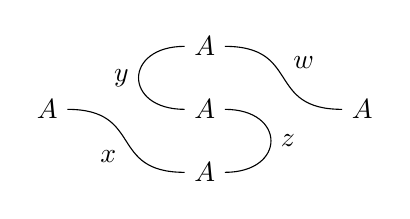
\begin{tikzpicture}[xscale=2,yscale=.8]
    \node (A1) at (0,0) {$A$};
    \node (A2a) at (1,1) {$A$};
    \node (A2b) at (1,0) {$A$};
    \node (A2c) at (1,-1) {$A$};
    \node (A3) at (2,0) {$A$};
    \draw (A1) to[out=0,in=180] node[auto,swap] {$x$} (A2c);
    \draw (A2a) to[out=0,in=180] node[auto] {$w$} (A3);
    \draw (A2a) to[out=180,in=180] node[auto,swap] {$y$} (A2b);
    \draw (A2b) to[out=0,in=0] node[auto] {$z$} (A2c);
  \end{tikzpicture}
\end{center}
or by solving a system of equations that ``unifies'' each arguments of the codomain $N(x,y,y)$ of $\phi$ with the corresponding argument of the domain $N(z,z,w)$ of $\psi$:
\begin{mathpar}
  x=z \and y=z \and y=w
\end{mathpar}

There are cases where this doesn't work; that is, pairs of extraordinary morphisms from $M$ to $N$ and from $N$ to $P$ that are ``non-composable'' despite having the same module $N$ in the middle.
For example, we might instead have
\begin{mathpar}
  \phi\in \mhom{M(x)}{N(x,y,y)} \and \xi\in\mhom{N(w,z,z)}{P(w)}.
\end{mathpar}
The problem here is that when ``composing components'' there is no way to decide what $y$ and $z$ should be: we can write down the composite
\[ M(x) \xto{\phi_{x,y,y}} N(x,y,y) \xto{\xi_{x,y,y}} P(x) \]
for any value of $y$, and there is no canonical choice (note that $x$ and $w$ might belong to an entirely different cat, so choosing $y=x$ is not an option).
Graphically, this problem is visible as the presence of a ``loop'':
\begin{center}
  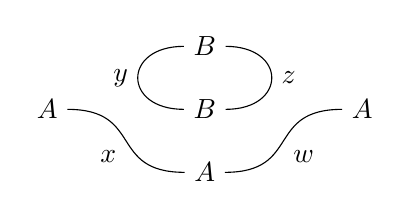
\begin{tikzpicture}[xscale=2,yscale=.8]
    \node (A1) at (0,0) {$A$};
    \node (A2a) at (1,1) {$B$};
    \node (A2b) at (1,0) {$B$};
    \node (A2c) at (1,-1) {$A$};
    \node (A3) at (2,0) {$A$};
    \draw (A1) to[out=0,in=180] node[auto,swap] {$x$} (A2c);
    \draw (A2c) to[out=0,in=180] node[auto,swap] {$w$} (A3);
    \draw (A2a) to[out=180,in=180] node[auto,swap] {$y$} (A2b);
    \draw (A2a) to[out=0,in=0] node[auto] {$z$} (A2b);
  \end{tikzpicture}
\end{center}
A more careful explanation of this condition, and a proof that it is the most general answer (for the classical case of enriched categories), can be found in~\cite{ek:gen-funct-calc}.

The technical work in the precise definition of a kit is to make precise \emph{all} the allowable composites of extraordinary morphisms, how they interact with restriction along functors, and in what sense these composites must be ``associative''.
However, in practical applications this generality is rarely needed, as most extraordinary morphisms only involve a few variables, and intuition from ordinary category theory is generally sufficient to give the right answer.
We intend to demonstrate this with some examples of doing ``formal category theory'' in a kit; but first we need to discuss some universal properties of cats and modules.

\section{Universal constructions}
\label{sec:univ}

Universal constructions in a kit are more complicated than those in an ordinary category, due to the interaction of the different kinds of morphisms.
Specifically, universal properties of cats generally have to be extended to say something about modules and module morphisms, while universal properties of modules have to include the extraordinary module morphisms somehow and also be stable under restriction along functors.

\subsection{Tensor products of cats and opposites}
\label{sec:tens-opp}

We begin with the simplest universal properties for cats: those that directly internalize the operations represented ``virtually'' by the multicategorical nature of functors.
For instance, a tensor product of cats $A,B$ should be a cat $A\otimes B$ with a functor $\chi:(A,B)\to A\otimes B$ through which any functor $(A,B)\to C$ factors uniquely.

However, this plain universal property, though it suffices to determine $A\otimes B$ uniquely up to isomorphism, is insufficient in several ways.
Firstly, as in the case of ordinary multicategories, it needs to apply to more general functors containing $(A,B)$ as only part of their domain.
Secondly, it needs to apply even in the contravariant case: functors $(A\o,B\o)\to C$ should factor through $(A\otimes B)\o$.
Thirdly, it needs to apply to modules as well: we should have $\modk(A\otimes B)\cong \modk(A,B)$, and similarly when other cats are also present.
And finally, it also needs to apply to module morphisms of all sorts, even extraordinary ones.

In order to state all of these universal properties precisely, we need some more notation.
\begin{itemize}
\item We will write $A\e$ to indicate either $A$ or $A\o$, and in this case we write $A\epbar$ for the other one ($A\o$ or $A$, respectively).
\item We will use the letter $\Gamma$ for a finite list of modules with abstract variables, such as $M(a,b),N(b,c,d),P(e)$ or $M_1(f(x),g(y,z)),M_2(h(y,x))$.
  Similarly, we will use the letter $\Omega$ for a single module with abstract variables; thus a general extraordinary module morphism can be written $\phi\in\mhom{\Gamma}{\Omega}$.
\item We will write $\subst\Gamma x \theta$ for the result of substituting the expression $\theta$ for all occurrences of the abstract variable $x$ in $\Gamma$, and similarly, for $\Omega$.
  Thus, for instance, if $\Omega = M(a,b)$, then $\subst\Omega a{f(x,y)} = M(f(x,y),b)$.
  Note that this might perform zero, one, or two substitutions, depending on how many times the variable occurs.
\end{itemize}

\begin{defn}\label{defn:tens-cat}
  A \textbf{tensor product} of cats $A,B$ is a cat $A\otimes B$ with a functor $\chi:(A,B) \to A\otimes B$ such that
  \begin{enumerate}
  \item Precomposition with $\chi$ induces bijections of functor sets
    \[ \K((\Psi,(A\otimes B)\e),C) \toiso \K((\Psi,A\e,B\e),C)\]
    for any list $\Psi$ of cats with variance;\label{item:tenscat-1}
  \item Restriction along $\chi$ induces an isomorphism of categories
    \[ \modk(\Psi,(A\otimes B)\e) \toiso \modk(\Psi,A\e,B\e) \]
    for any $\Psi$; and finally
  \item Restriction along $\chi$ induces bijections of sets of extraordinary morphisms
    \[ \mhomc{\Psi,z:(A\otimes B)\e}{\Gamma}{\Omega}\toiso \mhomc{\Psi,x:A\e,y:B\e}{\subst\Gamma z{\chi(x,y)}}{\subst \Omega z {\chi(x,y)}}\]
    whenever this makes sense.\label{item:tenscat-3}
  \end{enumerate}
\end{defn}

Note that due to the symmetric group actions, it suffices to assert these universal properties when $A\otimes B$ is at the end of a list; corresponding properties then follow when it appears anywhere.

We can similarly define $n$-ary tensor products of cats for all $n$, and using only~\ref{item:tenscat-1} we can show that these are associative and symmetric insofar as they exist.
That is, if $A\otimes B$ and $(A\otimes B)\otimes C$ exist, then the latter is a ternary tensor product; hence if $B\otimes C$ exists then $A\otimes (B\otimes C)$ exists and is isomorphic to $(A\otimes B)\otimes C$.
A 0-ary tensor product is a cat $I$ with a functor $\chi:()\to I$, precomposition with which induces isomorphisms
\begin{align*}
  \K((\Psi,I\e),C) &\toiso \K(\Psi,C)\\
  \modk(\Psi,I\e) &\toiso \modk(\Psi)\\
  \mhomc{\Psi,z:I\e}{\Gamma}{\Omega} &\toiso \mhomc{\Psi}{\subst\Gamma z\chi}{\subst\Omega z \chi}
\end{align*}
In particular, if all tensor products of cats exist, then the category $\K_1$ of cats and unary functors is symmetric monoidal.

Similarly, we can internalize contravariance by defining an operation of ``oppositization''.
We will write this as $(-)\op$ to distinguish it from the formal marker of contravariance $(-)\o$.

\begin{defn}\label{defn:opp-cat}
  An \textbf{opposite} of a cat $A$ is a cat $A\op$ with a functor $\chi:(A\o) \to A\op$ precomposition with which induces isomorphisms
  \begin{align*}
    \K((\Psi,(A\op)\e),C) &\toiso \K((\Psi,A\epbar),C)\\
    \modk(\Psi,(A\op)\e) &\toiso \modk(\Psi,A\epbar) \\
    \mhomc{\Psi,z:(A\op)\e}{\Gamma}{\Omega} &\toiso \mhomc{\Psi,x:A\epbar}{\subst\Gamma z {\chi(x)}}{\subst\Omega z{\chi(x)}}
  \end{align*}
\end{defn}

If all opposites exist, then $(-)\op$ defines an endofunctor of $\K_1$.
By comparing universal properties, we can see that $(A\op)\op\cong A$ and $(A\otimes B)\op \cong A\op \otimes B\op$ and $I\op$, so that $(-)\op$ is a ``symmetric monoidal involution'' in a suitable sense.


\subsection{Tensor products of modules}
\label{sec:tens}

Like the tensor product of cats, the tensor product of modules has a universal property very much like that of tensor products in an ordinary multicategory.
It is simpler in that we don't need to worry about the dependence of modules on cats (the second two properties in \cref{defn:tens-cat,defn:opp-cat}).
However, it is more complicated in that the universal property applies to all sorts of extraordinary morphisms, and that it must be stable under restriction along functors.

To state this precisely, we need a bit more notation.
\begin{itemize}
\item If $M\in\modk(\Psi)$, we will write $M(\theta)$ for $M$ with a list of expressions $\theta$ for its abstract variables.
  For instance, if $M\in\modk(A,B\o,C)$ and we have $g:X \to A$ and $h:(Y\o,Z)\to B$ and $k:()\to C$, then with $\theta=(g(x),h(y,z),k)$ we have $M(\theta) = M(g(x),h(y,z),k)$.
  We will also use letters like $\gamma$ and $\omega$ for such lists $\theta$.
\end{itemize}

\begin{defn}
  A \textbf{tensor product} of modules $M_1\in\modk(\Psi_1)$ and $M_2\in\modk(\Psi_2)$ is a module $M_1\otimes M_2 \in \modk(\Psi_1,\Psi_2)$ along with an (ordinary) morphism $\chi:(M_1,M_2)\to M_1\otimes M_2$ such that precomposition with $\chi$ (or some restriction of it) induces bijections
  \[ \mhom{\Gamma,(M_1\otimes M_2)(\theta_1,\theta_2)}{\Omega} \toiso \mhom{\Gamma,M_1(\theta_1),M_2(\theta_2)}{\Omega} \]
\end{defn}

The presence of the $\theta$s means that this universal property includes extraordinary morphisms of all sorts, where paired variables may occur anywhere.
Examples include:
\begin{align*}
  \mhom{(M_1 \otimes M_2)(a,b)}{N(a,b)} &\toiso \mhom{M_1(a), M_2(b)}{N(a,b)}\\
  \mhom{(M_1 \otimes M_2)(a,a)}{N} &\toiso \mhom{M_1(a), M_2(a)}{N}\\
  \mhom{P(a),(M_1 \otimes M_2)(a,b,c)}{N(b,c,d,d)} &\toiso \mhom{P(a),M_1(a,b), M_2(c)}{N(b,c,d,d)}\\
\intertext{
and so on.
Similarly, $\theta$ can also include restrictions, so that we might have}
  \mhom{(M_1\otimes M_2)(f(a),g(b))}{N(a,b)} &\toiso \mhom{M_1(f(a)),M_2(g(b))}{N(a,b)}
\end{align*}
In other words, the restricted morphism $(f,g)^*\chi : f^*M, g^*N \to (f,g)^*(M\otimes N)$ has the universal property that would be expected of $\chi: f^*M, g^*N \to f^*M \otimes g^*N$, and thus tensor products are stable under restriction: $ (f,g)^*(M\otimes N) \cong  f^*M \otimes g^*N$.

In general this stability is only up to isomorphism, so we technically ought to resist the temptation to write things like $M_1(a,b)\otimes M_2(c)$ instead of $(M_1 \otimes M_2)(a,b,c)$.
However, the former notation is so useful (it reminds us how the dependencies split) that we will often succumb to this temptation.
It should be possible to prove a coherence theorem making tensor products (and all similar universal properties to be introduced below) strictly stable under restriction, and this is moreover how they appear in the type theory of~\cite{lnss:dirtt}.
Remember also that the pairing of variables only indicates the type of extraordinary morphism under consideration; when we write $(M_1 \otimes M_2)(a,a)$ or $M_1(a)\otimes M_2(a)$ we are still talking about the same tensor product module $M_1\otimes M_2$, just different kinds of morphisms out of it.

As usual, we can define $n$-ary tensor products for all $n$, and the usual arguments show that these are associative and symmetric insofar as they exist.
A nullary tensor product is a module $I\in \modk(())$ and a morphism $() \to I$, precomposition with which induces bijections $\mhom{\Gamma,I}{\Omega} \toiso \mhom\Gamma \Omega$.

\subsection{Ends and coends}
\label{sec:ends-coends}

The tensor product of modules has a universal property that extends to extraordinary morphisms, but the universal morphism $(M,N)\to M\otimes N$ itself is an ordinary morphism.
Now we consider universal morphisms that are themselves extraordinary.
Perhaps the simplest of these are ends and coends.
First one more bit of notation:

\begin{itemize}
\item We will write $\xi$ for a $\theta$ that contains no functors or pairings, only a list of distinct abstract variables.
  In other words, $M(\xi)$ simply stands for a way to import $M$ into abstract variable notation, which is unique up to the choice of variable names.
  Thus if $M\in \modk(A,B\o,C)$ then $M(\xi)$ might mean $M(a,b,c)$ but not $M(g(x),h(y,z),k)$.
  Moreover, if different $\xi$s appear in an expression we assume them to be disjoint.
\end{itemize}

For instance, the universal morphism of a tensor product could be written in abstract variable notation as $\chi \in \mhom{M_1(\xi_1), M_2(\xi_2)}{(M_1\otimes M_2)(\xi_1,\xi_2)}$.
We avoided this before by writing it without abstract variables, but that is no longer possible now that we want to consider extraordinary universal morphisms.

\begin{defn}
  A \textbf{coend} of a module $M\in \modk(A,A\o,\Psi)$ is a module $\coend^A M\in\modk(\Psi)$ together with a morphism $\chi\in\mhom{M(a,a,\xi)}{\big(\coend^A M\big)(\xi)}$, precomposition with which induces bijections
  \[ \mhom{\Gamma,(\coend^A M)(\theta)}{\Omega} \toiso \mhom{\Gamma,M(a,a,\theta)}{\Omega} \]
  whenever this makes sense.
\end{defn}

If other variables belonging to $A$ occur elsewhere, then we may indicate which one is being ``coended'' by writing $\coend^{a:A} M(a,a)$.
In this notation the variable $a$ is ``bound'' and no longer indicates any ordinary or extraordinary dependence of the morphism under consideration.

The simplest case of the universal property of a coend is that
\[ \mhom{\coend^A M}{N} \cong \mhom{M(a,a)}{N} \]
for $M\in\modk(A,A\o)$ and $N\in\modk(())$.
In other words, $\coend^A M$ is the module universally equipped with a morphism from $M$ that is extraordinary in $A$.
As with tensor products, the full universal property also applies to multivariable morphisms that may have other variables, both ordinary and extraordinary, and also implies a stability under restriction: $f^*(\coend^A M) \cong \coend^A f^*M$.

This stability is, of course, only true for restriction along functors between \emph{other} cats that $M$ may depend on: a functor $f:B\to A$ does not induce an isomorphism $\coend^{B} (f,f)^* M \cong \coend^A M$.
We do, however, have a morphism $\coend^{B} (f,f)^* M \to \coend^A M$, induced by first restricting the universal morphism $M(a,a) \to \coend^A M$ along $f$ to obtain $M(f(b),f(b)) \to \coend^A M$, then applying the universal property of $\coend^B$.

By comparing universal properties, we can deduce the ``Fubini theorem''
\[ \coend^A \coend^B M \cong \coend^B \coend^A M. \]
Moreover, if $A\otimes B$ exists, then both iterated coends are also isomorphic to $\coend^{A\otimes B} M'$, where $M'$ corresponds to $M$ under the universal property of $A\otimes B$ (applied twice, once covariantly and once contravariantly).
Similarly, we have $\coend^I M'\cong M$ if $I$ is the unit cat and $M'$ corresponds to $M$ under its universal property.

Combining the coend with the (external) tensor product of modules, we obtain the \emph{binding} or \emph{canceling} tensor product of modules:
\[ M\otimes_A N = \coend^A (M\otimes N) \]
where $M\in\modk(\Psi_1,A)$ and $N\in\modk(\Psi_2,A\o)$ (or vice versa).
Comparing universal properties, we see that this is also associative:
\[ (M\otimes_A N) \otimes_B P \cong M\otimes_A (N\otimes_B P) \]
and we can verify the pentagon axiom.
This wants to be the composition operation in a bicategory of cats and modules, where the hom-category from $A$ to $B$ is $\modk(B\o,A)$; but we do not yet have the identity 1-cells for such a bicategory.

Note that it is possible to express directly the universal property of the binding tensor product: it comes with a morphism $M(\xi_1,a), N(a,\xi_2) \mto (M\otimes_A N)(\xi_1,\xi_2)$, inducing bijections
\[ \mhom{\Gamma,(M\otimes_A N) (\theta_1,\theta_2)}{\Omega} \toiso \mhom{\Gamma,M(\theta_1,a),N(a,\theta_2)}{\Omega} \]
This is useful because in some kits the binding tensor product may exist even if the external tensor product and coend do not separately exist.

Finally, ends are dual to coends.
These are our first module with a ``mapping in'' universal property.

\begin{defn}
  An \textbf{end} of a module $M\in \modk(A,A\o,\Psi)$ is a module $\tend_A M\in\modk(\Psi)$ together with a morphism $\chi\in\mhom{\big(\tend_A M\big)(\xi)}{M(a,a,\xi)}$, postcomposition with which induces bijections
  \[ \mhom{\Gamma}{(\tend_A M)(\theta)} \toiso \mhom{\Gamma}{M(a,a,\theta)} \]
  whenever this makes sense.
\end{defn}


\subsection{Function modules}
\label{sec:func-mod}

For ends and coends, the universal morphism is extraordinary in the input (the module being ended or coended); now we move on to universal morphisms that are extraordinary in the output (the object with a universal property).
The first of these are function modules, the ``right adjoints'' to tensor products --- although as we will see, to actually construct adjunctions requires incorporating ends and coends as well.

\begin{defn}
  A \textbf{function module} of modules $M_1\in \modk(\Phi_1)$ and $M_2\in \modk(\Phi_2)$ is a module $M_1\multimap M_2 \in \modk(\Phi_1\o,\Phi_2)$ with a morphism
  \[\ev \in \mhom{(M_1\multimap M_2)(\xi_1,\xi_2), M_1(\xi_1)}{M_2(\xi_2)},\]
  postcomposition with which induces bijections
  \begin{equation}
    \mhom{\Gamma}{(M_1\multimap M_2)(\theta_1,\theta_2)} \toiso
    \mhom{\Gamma,M_1(\theta_1)}{M_2(\theta_2)}\label{eq:func-ump}
  \end{equation}
  whenever this makes sense.
\end{defn}

As before, $\xi$'s represent disjoint lists of distinct variables; thus $\ev$ (``evaluation'') is a single morphism such as $(M_1\multimap M_2)(a,b), M_1(a) \mto M_2(b)$.
But also as before, the $\theta$'s represent arbitrary expressions, possibly with variable pairings; thus the universal property includes as particular cases:
\begin{align*}
  \mhom{N(a,b)}{(M_1\multimap M_2)(a,b))} &\toiso \mhom{N(a,b),M_1(a)}{M_2(b)}\\
  \mhom{N}{(M_1\multimap M_2)(a,a))} &\toiso \mhom{N,M_1(a)}{M_2(a)}\\
  \mhom{N(a,b)}{(M_1\multimap M_2)(a,c,b,c))} &\toiso \mhom{N(a,b),M_1(a,c)}{M_2(b,c)}\\
  \mhom{N(f(x,z),g(y))}{(M_1\multimap M_2)(h(x,y),z))} &\toiso \mhom{N(f(x,z),g(y)),M_1(h(x,y))}{M_2(z)}
\end{align*}
and so on.
Note that the composition map~\eqref{eq:func-ump} is indeed what we get by postcomposing with $\ev$: as described in \cref{sec:composing}, when composing $\mhom{(M_1\multimap M_2)(\xi_1,\xi_2), M_1(\xi_1)}{M_2(\xi_2)}$ with $\mhom{\Gamma}{(M_1\multimap M_2)(\theta_1,\theta_2)}$ (and technically the identity on $M_1(\xi_1)$ as well), $\xi_1$ and $\xi_2$ get identified with $\theta_1$ and $\theta_2$, so that in the result instead of $M_1(\xi_1)$ and $M_2(\xi_2)$ in the domain and codomain we have $M_1(\theta_1)$ and $M_2(\theta_2)$.

Combining the universal properties of function modules with tensor products, we have an isomorphism
\[ \mhom{(M_1\otimes M_2)(\theta_1,\theta_2)}{M_3(\theta_3)} \cong \mhom{M_1(\theta_1)}{(M_2\multimap M_3)(\theta_2,\theta_3)}
\]
that looks like an adjunction, except that one side or the other (or both) must always be extraordinary.
However, if we add in an end or a coend, we can make an isomorphism between two ordinary sets of morphisms, and therefore an actual adjunction.
Examples include
\begin{align*}
  \mhom{\coend^{a:A} (M_1\otimes M_2)(a,a)}{M_3} &\cong \mhom{M_1(a)}{(M_2\multimap M_3)(a)}\\
  \mhom{(M_1\otimes M_2)(a)}{M_3(a)} &\cong \mhom{M_1}{\tend_{a:A} (M_2\multimap M_3)(a,a)}\\
\end{align*}
which can be interpreted (for fixed $M_2\in \modk(A)$) as adjunctions
\begin{align*}
  \modk(A) &\leftrightarrows \modk(())\\
  \modk(()) &\leftrightarrows \modk(A)
\end{align*}
respectively.
Adding in a couple of other variables, we find that for $M\in \modk(B\o,A)$ and $N\in\modk(C\o,B)$ and $P\in modk(C\o,A)$ we have
\begin{align*}
  \mhom{\coend^{b:B} (N\otimes M)(c,b,b,a)}{P(c,a)} &\cong \mhom{M(b,a)}{\tend_{c:C} (N\multimap P)(c,b,c,a)}
\end{align*}
Since $\coend^B (N\otimes M)$ is the composition in the expected ``bicategory of profunctors'', this shows that if we have function modules and ends then that will be a \emph{closed bicategory}, in the usual sense that its composition functors have right adjoints on both sides.

As in the case of the binding tensor product, it is sometimes useful to directly name the \emph{binding function module}
\[ M\multimap_A N = \tend_A (M\multimap N)\]
whose universal property can be expressed directly as a morphism
\[\ev\in \mhom{(M\multimap_A N)(\theta_1,\theta_2),M(\theta_1,a)}{N(\theta_2,a)}\]
postcomposition with which induces an isomorphism
\[ \mhom{\Gamma}{(M\multimap_A N)(\theta_1,\theta_2)} \toiso
\mhom{\Gamma,M(\theta_1,a)}{N(\theta_2,a)}.
\]


\subsection{Hom-modules and representable modules}
\label{sec:hom}

The most important universal objects in a kit are the ``hom-modules'' $\mor A \in \modk(A\o,A)$.
Their universal property is essentially a ``two-sided double Yoneda lemma''.

\begin{defn}
  A \textbf{hom-module} of a cat $A$ is a module $\mor A \in \modk(A\o,A)$ together with a morphism $\id_A \in \mhom{}{\mor A(a,a)}$, precomposition with which induces bijections
  \[ \mhom{\Gamma,\mor A(x,y)}{\Omega} \toiso
  \mhom{\subst\Gamma y x}{\subst\Omega y x}
  \]
\end{defn}

Two instances of this universal property look like the Yoneda lemma and the co-Yoneda lemma:
\begin{align*}
  \mhom{\mor A(x,y)}{M(x,y)} &\toiso \mhom{}{M(x,x)}\\
  \mhom{M(x),\mor A(x,y)}{N(y)} &\toiso \mhom{M(x)}{N(x)}
\end{align*}
TODO: Derive the one-sided versions.


\subsection{Functor and presheaf cats}
\label{sec:func-pshf}


\section{Examples of formal category theory}
\label{sec:examples}

We will always assume that all kits have hom-modules; this seems to be a prerequisite for doing much of any formal category theory.
However, we will explicitly assume other universal objects when we need them.

\subsection{Limits and colimits}

Consider functors $d:D\to C$ and $l:()\to C$ (i.e.\ $l$ is an ``object'' of $C$), and a module $J\in\modk(D)$.
A \textbf{$J$-weighted cone} over $d$ with vertex $l$ is a (ordinary) module morphism
\[ \pi \in \mhom{J(x)}{\mor{C}(l,d(x))}. \]
Using the universal property of hom-modules, this corresponds to a morphism
\[ \pi' \in \mhom{\mor{C}(y,l),J(x)}{\mor{C}(y,d(x))}. \]
We say that $\pi$ exhibits $l$ as a \textbf{$J$-weighted limit} of $d$ if $\pi'$ gives $\mor C(1,l)$ the universal property of the binding function module $J \multimap_D \mor{C}(1,d)$; in other words, if postcomposition with $\pi'$ induces bijections
\[ \mhom{\Gamma}{\mor{C}(y,l)} \toiso \mhom{\Gamma,J(x)}{\mor{C}(y,d(x))}. \]
Of course, if $J \multimap_D \mor{C}(1,d)$ is known to exist (such as if $\K$ has ends and function modules), then to make $l$ a $J$-weighted limit of $d$ is equivalent to giving an isomorphism $\mor{C}(1,l) \cong J \multimap_D \mor{C}(1,d)$ in $\modk(C\o)$.

(Hmm, in the definition of function modules (and all the other universal properties) I incorporated a substitution to make it restriction-stable.  Is that necessary to do here too?  In an equipment that corresponds to asserting the universal property with respect to cells having nontrivial vertical-arrow boundaries.  But maybe we can avoid that once we have homs and the Yoneda lemma by moving them into the domain?)

While the above definition most closely matches the usual definition of weighted limits, it is not necessary to restrict $d$ and $l$ to have unary and nullary domains, respectively.
The case when $l$ also has unary domain $E$ is also very important.
In this case $\pi$ is ordinary in $E$ and $\pi'$ is extraordinary:
\begin{align*}
\pi &\in \mhom{J(e,x)}{\mor{C}(l(e),d(x))} \\
\pi' &\in \mhom{\mor{C}(y,l(e)),J(e,x)}{\mor{C}(y,d(x))}
\end{align*}
and the limit is again characterized by $\mor{C}(1,l) \cong J \multimap_D \mor{C}(1,d)$, only now this is an isomorphism in $\modk(C\o,E)$.
Since universal properties are stable under restriction, it follows that for any $f:E'\to E$ we have also $\mor{C}(1,l f) \cong J(f,1) \multimap_D \mor{C}(1,d)$, so that $l:E\to C$ is a functor given by taking ``pointwise limits''.

As a special case, we can define (pointwise) Kan extensions.
If $f:D\to C$ and $g:D\to E$ are functors, then the right Kan extension of $f$ along $g$ (if it exists) is the limit of $f$ weighted by $\mor{E}(1,g)$.

\part{The definition of a kit}
\label{part:def}

\section{Generalized polycategories}
\label{sec:genpoly}

Our formal definition of a kit will be a special case of a general notion called a \emph{generalized polycategory}.
Generalized polycategories appear only implicitly in the literature (e.g.~\cite{garner:polycats}), so we will have to define them as well along the way.
However, we defer their general study to a later paper, taking here a reasonably geodesic route to the definition of kit.

Roughly speaking, generalized polycategories are to polycategories as generalized multicategories are to multicategories.
Recall that a \emph{multicategory} is like a category in which a morphism can have a finite list of objects, rather than a single object, as its domain (but still only a single object as codomain).
\emph{Generalized multicategories} are a vast generalization obtained by observing that ``finite lists'' can be regarded as elements of the free-monoid monad, and that a version of the definition of multicategory can be carried out for \emph{any} sufficiently well-behaved monad.

\emph{Polycategories}, on the other hand, are like categories in which a morphism can have finite lists of objects as both its domain and codomain.
However, this brief description is significantly farther from a precise definition than the corresponding brief description of multicategories, because there are many more choices about how to allow such morphisms to be composed.
Polycategories proper~\cite{szabo:polycats,cs:wk-distrib} result from one such choice, but other (perhaps even more natural) choices yield structures such as ``colored props'' and ``colored properads''.\footnote{Thus perhaps the general notion should be called a ``generalized prop'', but ``generalized polycategory'' is more euphonious and intuitive-sounding.}

\emph{Generalized polycategories} are thus defined relative not just to two monads (one describing the domains and one the codomains), but also a ``distributive law'' between them that describes ``how morphisms should be composed''.
Ordinary polycategories were defined in this language by Garner~\cite{garner:polycats}; to obtain a general notion we abstract out the details of his construction (with some changes; see below).
This is promising as an avenue for defining kits, since we can use the distributive law to encode the ``allowable composites'' of extraordinary natural transformations.

There are a number of perspectives on generalized multicategories that one could enhance to a theory of generalized polycategories.
We will use the framework of~\cite{cs:multicats}, except that (aiming at a geodesic route to kits) we simplify it by considering only double categories rather than the ``virtual double categories'' used there.

Specifically, we consider \emph{pseudo double categories}, in which one direction of composition is strict and the other is only associative and unital up to isomorphisms in the strict direction.
The literature is not consistent about whether the strict direction is the ``vertical'' or the ``horizontal'' one.
To be agnostic about this, we will use instead the words \textbf{tight} and \textbf{loose} (from~\cite{ls:limlax}) for the strict and pseudo directions, and we allow ourselves to write them in either orientation, marking the loose morphisms with a dot to disambiguate.
Thus, a cell in a double category can be written either as
\[ \vcenter{\xymatrix{ A \ar[r]|{\bullet} \ar[d] \ar@{}[dr]|{\Downarrow}& B \ar[d] \\ C \ar[r]|{\bullet} & D } }
\qquad\text{or}\qquad
\vcenter{\xymatrix{ A \ar[d]|{\bullet} \ar[r] \ar@{}[dr]|{\Rightarrow}& C \ar[d]|{\bullet} \\ B \ar[r] & D } }
\]
We write $\circ$ for tight composition (of arrows or cells), and $\bcomp$ for loose composition (of arrows or cells).
Similarly, we write $1$ for tight identities (of objects or loose arrows), and $\hunit{A}$ for loose identities (of objects or tight arrows).

The particular double category we have most in mind is \dCat, whose objects are categories, tight arrows are functors, and loose arrows are profunctors.
We will also be interested in \emph{slice} double categories of \dCat: for any object $A$ of a double category \dD, in the slice $\dD/A$ the category $(\dD/A)_0$ of objects and tight maps is the slice of $\dD_0$ over $A$, and the category $(\dD/A)_1$ of loose arrows and cells is the slice of $\dD_1$ over $\hunit A$.

Between (pseudo) double categories we will be interested in \emph{lax functors}, which are lax in the loose direction and strictly functorial in the tight direction.
Lax functors admit an obvious notion of \emph{tight transformation}, with tight arrow components $\alpha_A:FA\to GA$ for each object $A$, and 2-cell components
\[ \vcenter{\xymatrix{ FA \ar[r]|{\bullet}^{FM} \ar[d]_{\alpha_A} \ar@{}[dr]|{\Downarrow}& FB \ar[d]^{\alpha_B} \\ GA \ar[r]|{\bullet}_{GM} & GB } } \]
for each loose arrow $A\xbto{M} B$.
This yields a strict 2-category of double categories.
By a \textbf{double monad} we mean a monad in this 2-category.

Distributive laws can also be defined internal to any 2-category; this yields a notion of \textbf{tight distributive law}.
However, for generalized polycategories we are interested in \emph{loose distributive laws}, which we now define.
If $F$ and $G$ are lax double functors between pseudo double categories, a \textbf{loose transformation} $\alpha:F\bto G$ consists of a loose arrow $\alpha_X : F X \bto G X$ for each object $X$ of the domain, forming a pseudonatural transformation between the loose parts of $F$ and $G$, together with for each tight arrow $f:X\to Y$ in the domain, a cell
\[ \xymatrix{ F X \ar[r]|-{\bullet}^-{\alpha_X} \ar[d]_{F f} \ar@{}[dr]|{\alpha_f} & G X \ar[d]^{G f} \\
F Y \ar[r]|-{\bullet}_-{\alpha_Y} & G Y} \]
satisfying some evident axioms; see~\cite{gp:something} wherein this is called a \emph{vertical transformation}.
These are the loose arrows in a double category of functors whose tight arrows are tight transformations, and whose cells are an evident kind of ``square modification''.

\begin{defn}\label{def:hdl}
  Let $T$ and $S$ be monads on a double category \K.
  A \textbf{loose distributive law} between $(T,\Tmult,\Tunit)$ and $(S,\Smult,\Sunit)$ consists of the following:
  \begin{enumerate}
    \item A loose transformation $\dl : T S \bto S T$.
    \item Square modifications
      \begin{mathpar}
        \xymatrix{ T T S \ar[r]|{\bullet}^{T \dl} \ar[d]_{\Tmult S}
          \ar@{}[drr]|{\Tdlmult} &
          T S T \ar[r]|{\bullet}^{\dl T} & S T T \ar[d]^{S \Tmult} \\
          T S \ar[rr]|{\bullet}_{\dl}&& ST}\and
        \xymatrix{ T S S \ar[r]|{\bullet}^{\dl S} \ar[d]_{T \Smult}
          \ar@{}[drr]|{\Sdlmult} &
          S T S \ar[r]|{\bullet}^{S \dl} & S S T \ar[d]^{\Smult T} \\
          T S \ar[rr]|{\bullet}_{\dl}&& ST}\and
        % \xymatrix{ & S \ar[dl]_{\Tunit S} \ar[dr]^{S \Tunit} \ar@{}[d]|{\Tdlunit} \\
        %   T S \ar[rr]|{\bullet}_{\dl} && S T}\and
        % \xymatrix{ & T \ar[dl]_{T\Sunit} \ar[dr]^{\Sunit T} \ar@{}[d]|{\Sdlunit} \\
        %   T S \ar[rr]|{\bullet}_{\dl} && S T}
        \xymatrix{ S \ar[d]_{\Tunit S} \ar[r]|{\bullet}^{\hunit S}  \ar@{}[dr]|{\Tdlunit} & S \ar[d]^{S \Tunit} \\
          T S \ar[r]|{\bullet}_{\dl} & S T}\and
        \xymatrix{ T \ar[d]_{T\Sunit} \ar[r]|{\bullet}^{\hunit T} \ar@{}[dr]|{\Sdlunit} & T \ar[d]^{\Sunit T}  \\
          T S \ar[r]|{\bullet}_{\dl} & S T}
      \end{mathpar}
      (These are versions of the diagrams that would have to \emph{commute} if $\dl$ were an ordinary tight distributive law.)
    \item The following equalities of square modifications hold:
      \begin{align*}
        \Tdlunit \circ \hunit{\Sunit} &= \Sdlunit \circ \hunit{\Tunit} \\ % PDA1
        \Sdlmult \circ (\Sdlunit S\bcomp \Sunit_\dl) &=  1_\dl \\ % PDA2
        \Sdlmult \circ (\dl_{\Sunit} \bcomp S \Sdlunit) &= 1_\dl \\ % PDA3
        \Tdlmult \circ (\Tunit_\dl \bcomp \Tdlunit T) &= 1_\dl \\    % PDA4
        \Tdlmult \circ (T\Tdlunit \bcomp \dl_{\Tunit}) &= 1_\dl \\  % PDA5
        \Sdlmult \circ (\Sdlmult S\bcomp \Smult_\dl) &= \Sdlmult \circ (\dl_{\Smult} \bcomp S \Sdlmult) \\ % PDA6
        \Tdlmult \circ (\Tmult_\dl\bcomp \Tdlmult T) &= \Tdlmult \circ (T \Tdlmult\bcomp \dl_{\Tmult}) \\ % PDA7
        \Sdlmult \circ (\Tdlunit S\bcomp S\Tdlunit) &= \Tdlunit \circ \hunit{\Smult} \\ % PDA8
        \Tdlmult \circ (T\Sdlunit\bcomp \Sdlunit T) &= \Sdlunit \circ \hunit{\Tmult} \\ % PDA9
        \Sdlmult \circ (\Tdlmult S\bcomp S\Tdlmult) &= \Tdlmult \circ (T\Sdlmult\bcomp \Sdlmult T) \circ \dlnat % PDA10
      \end{align*}
      where $\dlnat : \dl TS \bcomp TS \dl \toiso TS \dl \bcomp \dl TS$ is a pseudonaturality constraint of $\dl$.
      In all cases the tight naturality and monad axioms for the transformations $\Tmult,\Tunit,\Smult,\Sunit$ ensures that the boundaries of both sides of the equations agree automatically.
  \end{enumerate}
\end{defn}

The data and axioms of a loose distributive law may appear rather formidable when written out unforgivingly as above.
In \cref{fig:hdl-data,fig:hdl-axioms} we sketch them instead using an informal string diagram calculus, in which the monads $T$ and $S$ are written as a red and a blue string respectively and the loose transformation $\dl$ is a ``string crossing''.

\begin{figure}
  \centering
  \includegraphics{hdl-data.png}
  \caption{The data of a loose distributive law}
  \label{fig:hdl-data}
\end{figure}

\begin{figure}
  \centering
  \includegraphics[width=\textwidth]{hdl-axioms.png}
  \caption{The axioms of a loose distributive law}
  \label{fig:hdl-axioms}
\end{figure}

In~\cite{cs:genmulti} the theory of generalized multicategories relative to a double monad is developed in two steps, by first constructing a ``horizontal Kleisli virtual double category'' and then considering monoids therein.
In a later paper we will do the same for generalized polycategories relative to a loose distributive law, but at present it suffices to define the end result explicitly.

\begin{defn}
  Let $\dl : T S \bto S T$ be a loose distributive law between double monads.
  A \textbf{$\dl$-monoid} consists of an object $A$ and a loose arrow $M:TA\bto SA$ together with unit and multiplication cells
  \[ \xymatrix{
    A \ar[d]_{\Tunit_A} \ar[r]|{\bullet}^{\hunit A}  \ar@{}[dr]|{e\Downarrow} & A \ar[d]^{\Sunit_A} \\
    T A \ar[r]|{\bullet}_M & S A }\qquad
 \xymatrix{ TTA \ar[r]|{\bullet}^{T M} \ar[d]_{\Tmult_A} \ar@{}[drrr]|{m\Downarrow} &
    T S A \ar[r]|{\bullet}^{\dl} & S T A \ar[r]|{\bullet}^{S M} & S S A \ar[d]^{\Smult_A}\\
    T A \ar[rrr]|{\bullet}_M &&& S A}\]
  such that the two following two ways to compose the multiplication with the unit are equal (modulo unit constraints for loose composition) to the identity on $M$:
  \[ \xymatrix@C=1.7pc{
    TA \ar[r]|{\bullet}^{\hunit{T A}} \ar@{=}[d] \ar@{}[dr]|{\bar T} &
    TA \ar[r]|{\bullet}^{\hunit{TA}} \ar@{=}[d] 
    & TA \ar@{=}[d] \ar[r]|{\bullet}^{M} &
    SA \ar@{=}[d] \\
    TA \ar[r]|{\bullet}^{T\hunit A} \ar[d]_{T\Tunit_A} \ar@{}[dr]|{Te} &
    TA \ar[r]|{\bullet}^{\hunit{TA}} \ar[d]|{T\Sunit_A} \ar@{}[dr]|{\Sdlunit}
    & TA \ar[d]|{\Sunit_{TA}} \ar[r]|{\bullet}^{M} \ar@{}[dr]|{\eta_M} &
    SA \ar[d]^{\Sunit_{SA}} \\
    TTA \ar[r]|{\bullet}_{T M} \ar[d]_{\Tmult_A} \ar@{}[drrr]|{m} &
    T S A \ar[r]|{\bullet}_{\dl} & S T A \ar[r]|{\bullet}_{S M} & S S A \ar[d]^{\Smult_A}\\
    T A \ar[rrr]|{\bullet}_M &&& S A}
  \xymatrix@C=1.7pc{
    TA \ar@{=}[d] \ar[r]|{\bullet}^{M} &
    SA \ar@{=}[d] \ar[r]|{\bullet}^{\hunit{SA}} &
    SA \ar@{=}[d]  \ar[r]|{\bullet}^{\hunit{S A}} \ar@{}[dr]|{\bar S} &
    SA \ar@{=}[d]  \\
    TA \ar[d]_{\Tunit_{TA}} \ar[r]|{\bullet}^{M} \ar@{}[dr]|{\Tunit_M} &
    SA \ar[d]|{\Tunit_{SA}} \ar[r]|{\bullet}^{\hunit{SA}} \ar@{}[dr]|{\Tdlunit} &
    SA \ar[d]|{S\Tunit_A}  \ar[r]|{\bullet}^{S\hunit A} \ar@{}[dr]|{Se} &
    SA \ar[d]^{S\Sunit_A}  \\
    TTA \ar[r]|{\bullet}_{T M} \ar[d]_{\Tmult_A} \ar@{}[drrr]|{m} &
    T S A \ar[r]|{\bullet}_{\dl} & S T A \ar[r]|{\bullet}^{S M} & S S A \ar[d]^{\Smult_A}\\
    T A \ar[rrr]|{\bullet}_M &&& S A}\]
  and also the two following ways to compose the multiplication with itself are equal to each other:
  \[ \xymatrix@C=1.7pc{ TTTA \ar[r]|{\bullet}^{TTM} \ar[d]_{\Tmult T} \ar@{}[dr]|{\Tmult_M} &
    TTSA \ar[r]|{\bullet}^{T\dl} \ar[d]_{\Tmult S} \ar@{}[drr]|{\Tdlmult} & 
    TSTA \ar[r]|{\bullet}^{\dl T} &
    STTA \ar[r]|{\bullet}^{STM} \ar@{}[drrr]|{S m} \ar[d]^{S\Tmult} &
    STSA \ar[r]|{\bullet}^{S\dl} & 
    SSTA \ar[r]|{\bullet}^{SSM} & 
    SSSA \ar[d]^{S\Smult}\\
    TTA \ar[d]^{\Tmult} \ar@{}[drrrrrr]|{m} \ar[r]|{\bullet}_{TM} &
    TSA \ar[rr]|{\bullet}_{\dl} && 
    STA \ar[rrr]|{\bullet}_{SM} &&& SSA \ar[d]^{\Smult} \\
    TA \ar[rrrrrr]|{\bullet} &&&&&& SA}\]
  \[ \xymatrix@C=1.7pc{
    TTTA \ar[r]|{\bullet}^{TTM} \ar@{=}[d] &
    TTSA \ar[r]|{\bullet}^{T\dl} \ar@{=}[d] &
    TSTA \ar[r]|{\bullet}^{\dl T} \ar@{=}[d] \ar@{}[drr]|{\dlnat} &
    STTA \ar[r]|{\bullet}^{STM} &
    STSA \ar[r]|{\bullet}^{S\dl} \ar@{=}[d] & 
    SSTA \ar[r]|{\bullet}^{SSM} \ar@{=}[d] & 
    SSSA \ar@{=}[d]\\
    TTTA \ar[d]_{T\Tmult} \ar[r]|{\bullet}^{TTM} \ar@{}[drrr]|{T m} &
    TTSA \ar[r]|{\bullet}^{T\dl} &
    TSTA \ar[r]|{\bullet}^{TSM} &
    TSSA \ar[d]^{T\Smult} \ar[r]|{\bullet}^{\dl S} \ar@{}[drr]|{\Sdlmult} &
    STSA \ar[r]|{\bullet}^{S\dl} &
    SSTA \ar[d]_{\Smult T} \ar[r]|{\bullet}^{SSM} \ar@{}[dr]|{\Smult M} & SSSA \ar[d]^{\Smult S} \\
    TTA' \ar[d]^{\Tmult} \ar@{}[drrrrrr]|{m} \ar[rrr]|{\bullet}_{TM} &&&
    TSA \ar[rr]|{\bullet}_{\dl} && 
    STA \ar[r]|{\bullet}_{SM} & SSA \ar[d]^{\Smult} \\
    TA \ar[rrrrrr]|{\bullet} &&&&&& S A}\]
\end{defn}

TODO: Define the 2-category of $\dl$-monoids.

In the rest of the paper we will define a loose distributive law for which $\dl$-monoids are kits (or, more precisely, ``pre-kits'').
Of course, first we need a couple of monads.
In a kit there are actually \emph{four} different kinds of structure that have to be incorporated into these monads: the extraordinary pairing of variables in the domain, the extraordinary pairing in the codomian, the possibility of multiple modules in the domain, and the substitution of functor terms for abstract variables in the codomain.
To simplify the construction and clarify the essential point (composing extraordinary natural transformations), we will first define a loose distributive law for ``unary kits without substitution'' that includes only the first two; then we will add in the other two.

\section{Linear double monads}
\label{sec:linear-double-monads}

Many of the monads we will be interested in are particularly simple: they are the monads on a slice $\bCat/A$ induced by an internal category in \bCat (that is, a strict double category) with $A$ as object-of-objects.
In particular, their underlying functors are given by span composition.
Functors between slice categories of this sort are sometimes called \textbf{linear} (by analogy with the more general \emph{polynomial} functors that also involve an exponential); they and the ``linear'' transformations between them are induced by morphisms and 2-cells in the bicategory of spans in \bCat.

However, we need not only monads on the ordinary category \bCat, but on the double category \dCat; and also loose distributive laws between these.
For this it is convenient to have a structure that describes ``spans in \dCat'' analogous to the bicategory of spans in the 1-category \bCat.
There are several ways one could organize such a structure, but for us the important one will be the following.

Let \cDbl denote the 2-category of pseudo double categories and strong double functors.
This has finite products, so we can regard it as cartesian monoidal.

\begin{defn}[\cite{gg:lowdim-tricats}]
  A \textbf{locally cubical bicategory} is a \cDbl-enriched bicategory.
  Thus, it has objects with hom-double-categories $\iA(x,y)$, composition functors $\iA(y,z)\times \iA(x,y) \to \iA(x,z)$, unit functors $1\to \iA(x,x)$, and associativity and unitality tight natural isomorphisms satisfying the usual axioms.
  % We say that it is \textbf{normal} if the composition functors are normal (preserve identities up to isomorphism) and the unit functors $1\to \iA(x,x)$ are strong (preserve identities and composition up to isomorphism), and \textbf{strong} if the composition functors are also strong.
\end{defn}

We call the objects of $\iA(A,B)$ the \textbf{morphisms} of \iA and write them $A\oto B$.
We call the tight and loose arrows of $\iA(A,B)$ \textbf{tight 2-cells} and \textbf{loose 2-cells} of \iA, and write them as $A\to B$ and $A\bto B$ respectively, and we call the cells of $\iA(A,B)$ \textbf{3-cells} of \iA.
We refer to composition of tight 2-cells in $\iA(A,B)$ (and composition of 3-cells in the tight direction) as \textbf{transversal}, composition of loose 2-cells in $\iA(A,B)$ (and composition of 3-cells in the loose direction) as \textbf{vertical}, and the action of the composition functors $\iA(B,C)\times \iA(A,B) \to \iA(A,C)$ as \textbf{horizontal}.
We have in mind the following picture:
\begin{center}
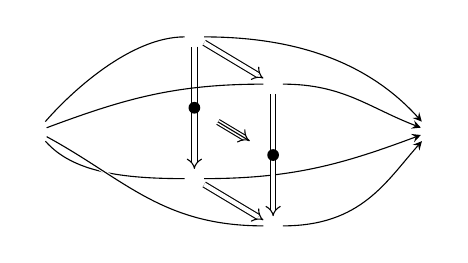
\begin{tikzpicture}[yscale=.6]
  \node (A) at (-1,0) {};
  \node (B) at (4,0) {};
  \node (y) at (2,1) {};
  \node (x) at (1,2) {};
  \node (z) at (1,-1) {};
  \node (w) at (2,-2) {};
  \draw[->] (A) to[out=60,in=-180,looseness=.7] (x) to[out=0,in=120] (B);
  \draw[->] (A) to[out=-60,in=-180] (z) to[out=0,in=-150] (B);
  \draw[white,very thick] (A) to[out=-40,in=-180] (w) to[out=0,in=-120] (B);
  \draw[->] (A) to[out=-40,in=-180] (w) to[out=0,in=-120] (B);
  \draw[darrow] (x) -- (y);
  \draw[darrow] (z) -- (w);
  \draw[barrow] (x) -- (z);
  \draw[barrow] (y) -- (w);
  \draw[darrow] (1.3,.2) -- (1.7,-.2); \draw (1.3,.2) -- (1.7,-.2);
  \draw[->] (A) to[out=30,in=-180] (y) to[out=0,in=150] (B);
\end{tikzpicture}
\end{center}

We write transversal composition with $\circ$ in functional order, vertical composition with $\bcomp $ in diagrammatic order, and horizontal composition with $\ocomp$ in diagrammatic order.
The unit functor $1:\iA(A,A)$ picks out an identity morphism $1_A$ for each object $A$.
In addition, every morphism $f$ has an identity tight 2-cell $1_f$ and an identity loose 2-cell $id_f$, every tight 2-cell $\alpha$ has an identity 3-cell $\id_\alpha$, every loose 2-cell $\beta$ has an identity 3-cell $1_\beta$, and we have $\id_{1_f} = 1_{\id_f}$.
We have $\id_f \ocomp \id_{g} \cong \id_{f\ocomp g}$ and $1_g \ocomp 1_g = 1_{f\ocomp g}$, as well as isomorphisms
\begin{equation}
  (p\ocomp q) \bcomp (r\ocomp s) \cong (p\bcomp r) \ocomp (q\bcomp s).\label{eq:interchange}
\end{equation}
Note also that the objects, morphisms, and tight 2-cells of a locally ax-cubical bicategory \iA form an ordinary bicategory under transversal and horizontal composition, which we denote $\cH(\iA)$.

There are two examples we care about.

\begin{eg}
  The cartesian monoidal 2-category \cDbl is in fact closed as a monoidal bicategory, i.e.\ the functors $\dA\times -$ have right biadjoints.
  As observed in~\cite{gg:lowdim-tricats}, it can therefore be regarded as a bicategory enriched over itself, i.e.\ a locally cubical bicategory.
  The hom-double-category $\fDbl(A,B)$ consists of strong double functors, tight transformations, loose transformations, and modifications between them.
\end{eg}

\begin{thm}
  There is a locally cubical bicategory $\cL(\dCat)$ described as follows.
  \begin{itemize}
  \item Its objects are groupoids.
  \item Its morphisms are spans $A \ot C \to B$ in \bCat such that $A$ and $B$ are groupoids and $C\to A$ is a fibration.
    Composition is by pullback, which is well-defined since fibrations are closed under pullback and composition.
  \item Its tight 2-cells are span morphisms:
    \[ \xymatrix@R=1pc{ & C \ar[dl] \ar[dr] \ar[dd] \\ A && B \\ &D \ar[ul] \ar[ur] } \]
    Thus the underlying bicategory is a sub-bicategory of $\cSpan(\bCat)$.
  \item Its loose 2-cells from $A \ot C \to B$ to $A\ot D \to B$ are profunctors $C\bto D$ equipped with a span of 2-cells in \dCat:
    \[ \xymatrix{ A \ar[d]|{\bullet}_{\hunit A} \ar@{}[dr]|{\Leftarrow} &
      C \ar[l] \ar[d]|{\bullet} \ar[r] \ar@{}[dr]|{\Rightarrow} &
      B \ar[d]|{\bullet}^{\hunit B}\\
      A & D \ar[l] \ar[r] & B. } \]
    These are composed by pullback in $\dCat_1$.
  \item Its 3-cells are span morphisms in $\dCat_1$.
  \end{itemize}
\end{thm}
\begin{proof}
  Recall from~\cite{gp:intercategories-i,gp:intercategories-ii} that an ``intercategory'' is an internal category in the 2-category \lxdbl of double categories and \emph{lax} double functors whose source and target functors are strict.
  Thus, a locally lax-cubical bicategory is an intercategory whose double category of objects is discrete and whose compostion and unit functors are strong.

  If an intercategory has strictly unital vertical composition (which can usually --- though not always --- be obtained by redefining vertical composition at identities), then we can discard all the arrows and cells in its double category of objects to obtain another intercategory with a discrete double category of objects.
  Applying this to the example of~\cite[6.5]{gp:intercategories-ii}, we get a structure that is almost like a locally cubical bicategory, but its composition functors are only lax normal rather than strong (though its unit functor is strong).
  However, when we restrict the objects to groupoids and the spans to have one leg a fibration, then the composition functor becomes strong as well, by \cite[Proposition 49]{garner:double-clubs}.
\end{proof}

Now, a linear functor $\bC/A\to \bC/B$ induced by a span $A \ot C \to B$ in $\bC$ can be described in terms of the bicategory $\cSpan(\bC)$, by identifying $\bC/A$ with the hom-category $\cSpan(\bC)(1,A)$ and composing them with the given span $A \ot C \to B$.
We can do something similar in $\cL(\dCat)$, where the slice double category $\dCat/A$ can be identified with the hom-double-category $\cL(\dCat)(1,A)$.
The following observation is entirely straightforward.

\begin{thm}
  Any object $X$ in a locally cubical bicategory \iA induces a representable locally cubical pseudofunctor $\iA(X,-):\iA \to \fDbl$.\qed
\end{thm}

In particular, any ``horizontal monad'' on $A\in \iA$ (whose multiplication and unit are tight 2-cells) induces a strong double monad on any hom-double-category $\iA(X,A)$.
Taking $\iA=\cL(\dCat)$ and $X=1$, we see that \emph{any linear monad on $\bCat/A$ induces a strong double monad on $\dCat/A$}.
(In a later paper we will show that something similar is true for all polynomial monads.)

The punchline is that loose distributive laws are also a ``locally cubical'' concept, i.e.\ they can be defined in any locally cubical bicategory and are preserved by locally cubical pseudofunctors.
To see this, simply take the definition and replace functors by 1-cells, tight and loose transformations by tight and loose 2-cells, square modifications by square 3-cells, and so on; the pseudonaturality of $\dl$ is replaced by the invertible interchange.
In particular, therefore, to define a loose distributive law between monads on a slice double category $\dCat/A$, it suffices to define a corresponding structure on $A$ in $\cL(\dCat)$.


\section{Extraordinary naturality}
\label{sec:extranat}

Let $V$ be the monad on $\bCat$ whose algebras are symmetric strict monoidal categories equipped with a strict symmetric monoidal strict involution, i.e.\ a strict symmetric monoidal functor $(-)\o : \C\to\C$ such that $(a\o)\o =a$ functorially.
Concretely, the objects of $V\C$ are finite lists of objects of $\C$, some of which are marked with a formal $(\blank)\o$, such as $(a,b\o,b,c\o,a)$.
It will also sometimes be convenient to write such a list as $(a\p,b\m,b\p,c\m,a\p)$, where $a\p=a$ and $a\m=a\o$; we can then write $a\e$ to mean either $a\p$ or $a\m$ depending on whether $\varepsilon=+$ or $\varepsilon=-$.
We write $\varepsilon^*$ for the reversed variance, i.e.\ $+^*=-$ and $-^*=+$.

Since $V\C$ is monoidal with an involution, its objects can be concatenated and oppositized (by distributing the opposite over the list), so for instance
\[(a,b\o)(c\o,d,a) = (a,b\o,c\o,d,a) \quad\text{and}\quad (b\o,a,a)\o = (b,a\o,a\o).\]
Its unit object is $\one = ()$.
The morphisms of $V\C$ are given by finite lists of morphisms of $\C$ labeled by permutations which respect the opposites, e.g.\ a morphism $(a,b\o,b,c\o,a) \to (d,e,d\o,f,e\o)$ might be:
\begin{tikzc}
  \node (A1) at (0,3) {$a$};
  \node (Bo2) at (1,3) {$b\o$};
  \node (B3) at (2,3) {$b$};
  \node (Co4) at (3,3) {$c\o$};
  \node (A5) at (4,3) {$a$};
  \node (D1') at (0,0) {$d$};
  \node (B2') at (1,0) {$e$};
  \node (Do3') at (2,0) {$d\o$};
  \node (C4') at (3,0) {$f$};
  \node (Ao5') at (4,0) {$e\o$};
  \draw[->] (A1) to[out=-90,in=90] node[ed,swap,pos=.2] {$f$} (B2');
  \draw[->] (Bo2) to[out=-90,in=90] node[ed,swap,pos=.1] {$g\o$} (Ao5');
  \draw[->] (B3) to[out=-90,in=90] node[ed,swap,pos=.9] {$h$} (D1');
  \draw[->] (Co4) to[out=-90,in=90] node[ed,swap,pos=.8] {$k\o$} (Do3');
  \draw[->] (A5) to[out=-90,in=90] node[ed,pos=.2] {$\ell$} (C4');
\end{tikzc}
Here $f:a\to e$, $g:b\to e$, $h:b\to d$, $k:c\to d$, and $\ell:a\to f$ are morphisms in $\C$.
Note that there can only be a morphism between two lists if they have the same length \emph{and} the same number of opposites.
Formally, if $A=(a_1\e[1],\dots,a_n\e[n])$ and $B=(b_1\ph[1],\dots,b_n\ph[n])$, then a morphism $A\to B$ is a pair $(\sigma,f)$ where $\sigma\in \Sigma_n$ is a permutation such that $\varphi_{\sigma(k)} = \varepsilon_{k}$, and $f=(f_1,\dots,f_n)$ is a list of morphisms with $f_n : a_n \to b_{\sigma(n)}$.

For the rest of this section, let \C be a \emph{discrete} category, whose objects will be the cats of our unary kit.
In particular, therefore $V\C$ is a groupoid.
We will define a loose distributive law on $V\C$ in $\fSpan(\dCat)$, inducing one on $\dCat/V\C$ whose generalized polycategories are ``unary kits without functors''.

The two monads involved in this distributive law will in fact be the same monad, which we denote $R$.
Being a horizontal monad in $\fSpan(\dCat)$, it is equivalently a monad in the bicategory $\cSpan(\bCat)$, i.e.\ an internal category in \bCat, i.e.\ a \emph{strict} double category $\dR$.
Since its category of objects $\dR_0$ is $V\C$, its objects are those of $V\C$ and its tight morphisms are the morphisms of $V\C$.
We now define its loose morphisms and cells.

Let us call an object of $V\C$ \textbf{totally covariant} if it contains no $(-)\o$'s.
A \textbf{$B$-trivial pre-matching} between $A,B\in V\C$ is an isomorphism $A \cong B E E\o$ in $V\C$ where $E$ is totally covariant and the permutation preserves the relative order of cats in $B$.
Two pre-matchings are \textbf{equivalent} if they are related by an isomorphism $E\cong E'$ (necessarily unique if it exists); a \textbf{$B$-trivial matching} is an equivalence class of $B$-trivial pre-matchings.
[Is this passage to equivalence classes the right thing to do?  Does it actually make sense everywhere?]

Now a loose morphism from $A$ to $B$ in our double category (an object of $\dR_1$) is a $B$-trivial matching between $A$ and $B$.
The loose composite of matchings $A\cong B D D\o$ and $B \cong C E E\o$ is the composite
\[ A\cong B D D\o \cong C E E\o D D\o \cong C (E D) (E D)\o. \]
The identity matching is the unique one with $E=()$.
The cells are commutative squares of two matchings and two isomorphisms, in an obvious sense.

This completes the definition of a strict double category $\dR$ with $\dR_0 = V\C$.
Note that the source and target functors of \dR are both individually fibrations (though the functor $(s,t):\dR_1 \to \dR_0\times \dR_0$ is not a fibration).
Thus, in particular it is a monad in $\cL(\dCat)$, and thus induces a strong double monad $R$ on $\dCat/V\C$.

An object of $\dCat/V\C$ is a functor $\E\to V\C$, where the fiber $\E(A)$ over $A=(a_1\e[1],\dots,a_n\e[n])$ is the set of modules with boundary $A$.
Usually we will assume it to be a discrete fibration (or equivalently a discrete opfibration, since $V\C$ is a groupoid), meaning that we can permute the cats in the boundary of a module.
The objects of $R\E$ are then obtained by choosing an object of $\E$, pairing up some of the cats in its boundary into covariant and contravariant pairs, and removing them from the boundary of the result.
Note that the passage from pre-matchings to matchings means that there is no ordering imposed on the paired cats, and $B$-triviality means that the order of the unremoved cats is maintained.
However, $R\E\to V\C$ is still no longer a \emph{discrete} fibration: an object in the fiber over $B$ consists of a $B$-trivial matching $A\cong BEE\o$ together with an object of $\E(A)$, and if $E$ admits automorphisms then so can such objects.

Now a profunctor $\cM:R\E \bto R\E$ in $\dCat/V\C$ consists of a set of ``morphisms'', each of which is assigned a pair of modules with some of their cats paired up to be its domain and codomain, plus a permutation relating the \emph{unpaired} cats in the domain and the codomain.
The latter datum is the 2-cell
\[ \xymatrix{ R\E \ar[d]|{\bullet}_{\cM} \ar[r] \ar@{}[dr]|{\Rightarrow} & V\C \ar[d]|{\bullet}^{\hunit {V\C}} \\ R\E \ar[r] & V \C } \]
exhibiting $\cM$ as a loose morphism in $\dCat/V\C$.
These elements of \cM are the extraordinary morphisms between modules, with the pairings in their domain and codomain representing the extraordinary-natural cats.
The profunctorial action means that the cats in the domains and codomains of morphisms can be permuted, including the extraordinary natural ones.

Now we have to define a loose distributive law of $R$ over itself on $\dCat/V\C$.
As suggested in \cref{sec:linear-double-monads}, we will do this by defining a loose distributive law of $\dR$ over itself in the locally cubical bicategory $\cL(\dCat)$.
For clarity, we write $\dS=\dT=\dR$, with \dS as a mnemonic for source and \dT for target; thus our goal is $\dl : \dT \ocomp \dS \bto \dS \ocomp \dT$.

Now $\dT\ocomp \dS$ and $\dS\ocomp \dT$ are spans from $V\C$ to itself, whose objects consist of a $B$-trivial matching $A\cong B D D\o$ and a $C$-trivial matching $B \cong C E E\o$, with the projections selecting $A$ and $C$.
Of course these have a composite $C$-trivial matching from $A$ to $C$; the additional data beyond the composite is simply a division of the paired cats into those in $D$ and those in $E$.
The object $B\in V\C$ is actually determined once we know $D$ and the composite, by $B$-triviality of the first matching.
In particular, the fibers of $\dT\ocomp \dS \to V\C \times V\C$ are discrete.

Our $\delta$ is supposed to be a profunctor $\dT \ocomp \dS \bto \dS \ocomp \dT$, which moreover must be a loose 2-cell in $\cL(\dCat)$ and thus come with cells
\[ \xymatrix{ V\C \ar[d]|{\bullet}_{\hunit {V\C}} \ar@{}[dr]|{\Leftarrow} &
  \dT\ocomp \dS \ar[l] \ar[d]|{\bullet} \ar[r] \ar@{}[dr]|{\Rightarrow} &
  V\C \ar[d]|{\bullet}^{\hunit {V\C}}\\
  V\C & \dS\ocomp\dT \ar[l] \ar[r] & V\C. } \]
Taken together, this means that for any $A,C$ and $A',C'$, and isomorphisms $A\cong A'$ and $C\cong C'$, plus a $C$-trivial matching from $A$ to $C$ and a $C'$-trivial matching from $A'$ to $C'$, both with the paired cats partitioned into two subsets, we must have a specified ``set of ways to compose''.
Put differently, the ``type'' of an element of $\dl$ is given by the following data:
\begin{equation}
  \xymatrix{ A \ar[d]_\cong \ar[r]^-\cong & B D D\o \ar[r]^-\cong & C E E\o D D\o & C \ar[d]^\cong \\
    A' \ar[r]_-\cong & B' D' (D')\o \ar[r]_-\cong & C' E' (E')\o D' (D')\o & C' }\label{eq:dl-type-1}
\end{equation}
Note that the isomorphism $C\cong C'$ is not required to ``commute'' with the others.

In fact, any such ``type'' will be inhabited by \emph{at most one} element of $\dl$.
It is simplest to describe the conditions under which this happens as a partial function from the left half of the diagram $B D D\o \cong A\cong A' \cong B' D' (D')\o$ to the right half.
Regard this composite isomorphism $B D D\o \cong B' D' (D')\o$ as a bipartite graph, and add additional edges connecting each cat in $D$ or $D'$ to its counterpart in $D\o$ or $(D')\o$.
In the resulting graph all vertices have degree 1 or 2, so it is a disjoint union of paths and cycles.
The partial function is defined if and only if there are \emph{no} cycles.
In this case, each path must start and end at a cat in $B$ or $B'$.
Every path that connects two cats in $B$ gives us an element of $E$, while every path that connects two cats in $B'$ gives us an element of $E'$.
The remaining paths connect one cat in $B$ with one in $B'$, specifying the isomorphism $C\cong C'$.
Note that the variance gets flipped every time a path ``changes direction'', so $E$- and $E'$-paths do indeed connect two copies of a cat with opposite variance, while the remaining ones preserve variance.

To be a profunctor, $\dl$ must also be acted on by permutations on both sides, compatibly with the projections to $\hunit{V\C}$ on both sides; but this is evident.
Thus, we have defined a loose 2-cell $\dl : \dT \ocomp \dS \bto \dS \ocomp \dT$ in $\cL(\dCat)$.

For the remaining data and axioms of a loose distributive law, we note that \dT and \dS play entirely symmetrical roles in the construction.
Thus, we can cut our work almost in half by symmetry (``almost'' because two of the axioms are self-dual under this symmetry).

[TODO \dots]


\section{Substitutions}
\label{sec:substitutions}

Next we incorporate nontrivial functors into our unary kits.
We start by describing the structure formed by the cats and functors as a kind of generalized multicategory in its own right.

We extend $V$ to a monad on the double category \dCat in the usual way (in fact, the unique way), by treating the elements of profunctors as if they were ``morphisms''.
That is, the above diagram could also represent an element of a profunctor $V H : V \D \hto V \C$, if $a,b,c\in\C$ and $d,e,f\in \D$ while $f\in H(a,e)$, $g\in H(b,e)$, and so on.
The technology of generalized multicategories then yields a notion of \emph{virtual $V$-algebra}, which contains ``multimorphisms'' whose domain is a list with variance like $(a,b\o,b,c\o,a)$.
Note that these are like symmetric multicategories in that symmetric groups act on the domain lists.

As usual, any virtual $V$-algebra \C generates a free $V$-algebra \Chat, whose objects are the lists with variance of objects in \C, and whose morphisms are lists of multimorphisms in \C, with domain and codomain arbitrarily permuted.
More precisely, a morphism from $A=(a_1\e[1],\dots,a_n\e[n])$ to $B=(b_1\ph[1],\dots,b_m\ph[m])$ in \Chat is represented by a pair $(\sigma,f)$ where $\sigma$ is a bijection $\left(\sum_{i=1}^m k_i\right) \toiso n$ and $f=(f_1,\dots,f_m)$ is a list of morphisms $f_i:(a_{\sigma(i,1)}\phe{i}{\sigma(i,1)},\dots,a_{\sigma(i,k_i)}\phe{i}{\sigma(i,k_i)}) \to b_i$.
(Here $\phe{i}{\sigma(i,j)}$ means the usual multiplication of signs.)
We quotient these pairs by the inner symmetric group actions, i.e.\ given permutations $\tau_i\in\Sigma_{k_i}$ we have $(\sigma(\sum_i \tau_i), f) = (\sigma,f\tau)$, where $(f\tau)_i = f_i \tau_i$ is defined by the symmetric action on the domains of morphisms in \C.
More formally, the hom-profunctor of \Chat is given by $\hom_{\Chat} = V\hom_\C \otimes_{VV\C} V\C(1,\Tmult)$.
Since the monoidal structure on \Chat is induced by the concatenation monoidal structure on $V\C$, we also write it as juxtaposition.

Note that every isomorphism in \Chat consists only of unary arrows.
By a \textbf{permutation isomorphism} in \Chat we mean an isomorphism in which these unary arrows are all identities; thus it really is nothing but a permutation.
In fact, the subcategory of permutation isomorphisms in $\Chat$ is isomorphihc to $V\C_0$, where $\C_0$ is the set of objects of $\C$.

Now fix a virtual $V$-algebra \C, whose objects will be our cats and functors.
We define a new linear double monad incorporating restriction along morphisms in \C as follows.
Say that a \textbf{pre-matching with restriction} between $A,B\in V\C$ is a morphism $B E E\o \to A$ in $\C$ where $E$ is totally covariant.
Two such pre-matchings are \textbf{equivalent} if they are related by an isomorphism $E\cong E'$ (necessarily unique if it exists); a \textbf{matching with restriction} is an equivalence class of pre-matchings.

Now let \dC be the strict double category whose tight morphisms are the permutation isomorphisms (that is, $\dC_0 = V\C_0$), whose loose morphisms from $A$ to $B$ are matchings with restrictions from $B$ to $A$, and whose cells are commutative squares in $\Chat$.
[Hmm, does this make sense with the passage to equivalence classes?]
Then \dC is a monad in $\cT(\dCat)$ on $V\C_0$.
We will construct a loose distributive law $\dC \ocomp \dS \to \dS\ocomp \dC$ in $\cL(\dCat)$, analogous to the one constructed in the previous section.

As a loose 2-cell in $\cL(\dCat)$, this will look like
\[ \xymatrix{ V\C_0 \ar[d]|{\bullet}_{\hunit {V\C_0}} \ar@{}[dr]|{\Leftarrow} &
  \dC\ocomp \dS \ar[l] \ar[d]|{\bullet} \ar[r] \ar@{}[dr]|{\Rightarrow} &
  V\C_0 \ar[d]|{\bullet}^{\hunit {V\C_0}}\\
  V\C & \dS\ocomp\dC \ar[l] \ar[r] & V\C_0. } \]
Now the ``type'' of an element of $\dl$ is given by the following data, in which some of the isomorphisms from~\eqref{eq:dl-type-1} have been replaced by morphisms in $\Chat$:
\[ \xymatrix{ A \ar[d]_\cong \ar[r]^-\cong & B D D\o & C E E\o D D\o \ar[l] & C \ar[d]^\cong \\
   A' & B' D' (D')\o \ar[l] \ar[r]_-\cong & C' E' (E')\o D' (D')\o & C' }\]
As before, any such ``type'' will be inhabited by at most one element of $\dl$, and we can describe the conditions under which this happens as a partial function from the left half of the diagram to the right half.
Thus, suppose given the left half, including in particular a composite morphism $B' D' (D')\o \to A'\cong A \cong B D D\o$ in $\Chat$.
By definition of $\Chat$, this consists of a morphism $f_b:F_b \to b$ of \C for each $b\in B$ and two morphisms $g_d:G_d\to d$ and $h_d:H_d \to d$ for each $d\in D$, together with an isomorphism
\begin{equation}\label{eq:subiso}
  B' D' (D')\o \toiso F_{b_1}\e[1]\cdots F_{b_n}\e[n] G_{d_1}\cdots G_{d_m} H_{d_1}\o \cdots H_{d_m}\o
\end{equation}
The conditions are then:
\begin{enumerate}
\item $g_d = h_d$ for each $d$ (and in particular, $G_d = H_d$).
\item Regard the isomorphism~\eqref{eq:subiso} as a bipartite graph, and add additional edges connecting each cat in $D$ to its counterpart in $D\o$, and each cat in each $G_d$ to its counterpart in $H_d\o$ (which is equal to $G_d\o$).
  Again this is a disjoint union of paths and cycles, and we require that there are no cycles.
\end{enumerate}
When these conditions hold, each path in the above graph must start and end at a cat in $B'$ or some $F_b$.
Every path that connects two cats in $B'$ gives us an element of $E'$, and we define $C'$ to be the remaining cats in $B'$, giving the matching $B' \cong C' E' (E')\o$.
Every path that connects two cats in some $F_b$'s (perhaps for different $b$'s) gives us an element of $E$, and we define $C$ to be the remaining cats in any of the $F_b$'s.
This yields an isomorphism $C E E\o \cong F_{b_1}\e[1]\cdots F_{b_n}\e[n]$, and we define the morphism $C E E\o \to B$ to be given by this isomorphism together with the $f_b$'s.
Finally, the remaining paths in the graph connect one cat in $B'$ with one in some $F_b$, specifying the isomorphism $C\cong C'$.
As before, the actions of permutation isomorphisms are trivial, so we have a loose 2-cell in $\cL(\dCat)$.

[TODO\dots]

% Each ``module'' will depend on a list of objects of \C with variance, i.e.\ an object of \Chat, and we can restrict modules along functors.
% Thus, to start with we take the modules to be a functor $\E:\Chat\op\to \bCat$.
% For the present we consider only strict functors here; there is probably no serious obstacle to weakening this, but the technical complications would be greater.
% Moreover, as is well-known any pseudofunctor can be strictified; and in many examples the functor is already strict.

% The morphisms in the categories $\E(B)$ will be the ``ordinary'' natural transformations.
% To describe the extraordinary ones, we will enhance \E to a generalized polycategory.
% Consider the equipment $\dCat^{\Chat\op}$, whose objects are (strict) functors $\E:\Chat\op\to\bCat$, whose vertical arrows are (strict) natural transformations, and so on.
% Note that the objects of $\dCat^{\Chat\op}$ can be regarded as split fibrations over $\Chat$ or as split opfibrations over $\Chat\op$, and similarly for the rest of its structure.

% \begin{rmk}
%   A functor $\Chat\op\to\bSet$ can equivalently be regarded as a horizontal arrow $1\hto \C$ in the virtual equipment of $V$-monoids.
%   (We owe this observation to Peter LeFanu Lumsdaine.)
%   Therefore, the equipment $\dCat^{\Chat\op}$ can also be regarded as the equipment of \emph{internal} categories in the category whose objects are such horizontal arrows.
% \end{rmk}

% We define a monad $S$ on $\dCat^{\Chat\op}$ by the following pullback:
% \[ \xymatrix{ S \E \ar[r] \ar[d] \pullback & \E \ar[d] \\
%   \Chat\times\Chat \ar[r]^-m \ar[d]^{\pi_2} & \Chat \\
%   \Chat }\]
% Here we regard \E as a split fibration over \Chat, the functor $m$ is defined by $m(A,B) = A A\o B$, and $\pi_2$ denotes the second projection.
% In other words, the objects of $S\E(B)$ are pairs $(A,M)$ where $A\in\Chat$ and $M\in\E(A A\o B)$, and its morphisms are pairs $(f,\phi) : (A,M)\to (A',M')$ with $f:A\to A'$ and $\phi : M \to f^*M'$.

% The unit $\E\to S\E$ sends $M\in \E(B)$ to $(\one,M)$; this is well-typed since $\Chat$ is strict monoidal, so $\one\one\o B = B$.
% The multiplication $SS\E\to S\E$ sends $(A,(B,M)) \in S S \E(C)$ to $(AB,\sigma^* M)\in S\E(E)$, where $\sigma : ABA\o B\o C \toiso A A\o B B\o C$ is the obvious permutation.
% The monad laws follow straightforwardly, though here we use the splitness of \E; if \E were only a pseudofunctor then $S$ would be only a pseudomonad.

% We define a monad $T$ on $\dCat^{\Chat\op}$ analogously, but regarding \E as a split opfibration over $\Chat\op$ instead:
% \[ \xymatrix{ T \E \ar[r] \ar[d] \pullback & \E \ar[d] \\
%   \Chat\op\times\Chat\op \ar[r]^-m \ar[d]^{\pi_2} & \Chat\op \\
%   \Chat\op }\]
% Thus, the objects of $T\E(B)$ are the same as those of $S\E(B)$, while its morphisms are pairs $(f,\psi) : (A,M)\to (A',M')$ with $f:A'\to A$ and $\psi : f^* M \to M'$.

% Now we have come to the heart of the definition: we will construct a horizontal distributive law $\delta : TS \hto ST$ that encodes the ``loop-free string-diagram compositions'' allowed for extranatural transformations.
% The resulting generalized polycategories will contain an object $\E\in \dCat^{\Chat}$, describing the modules and ordinary natural transformations as before, and also a horizontal arrow $\cM: T\E \hto S\E$, describing the extraordinary natural transformations.
% Here the ``poly-arrows'' from $(A,M)$ to $(C,N)$ over $B\in\Chat$ will represent transformations of the form $M(a,a,b) \to N(c,c,b)$, ordinary-natural in $b$ and extraordinary-natural in the two possible ways in $a$ and $c$.
% Note that here $(A,M)\in S\E$ and $(B,N)\in T\E$; as a mnemonic $S$ stands for ``source'' and $T$ for ``target''.

% (Note that since $A,B,C$ are objects of $\Chat$, hence lists of objects of \C with variance, we are actually allowing ordinary and extraordinary naturality in arbitrarily many variables.)
% In a later section we will further ``mix in'' the monad for symmetric monoidal categories to this distributive law, further enhancing these generalized polycategories to allow multiple objects in the domains of arrows.

% The fact that the poly-arrows form a horizontal arrow \cM in $\dCat^{\Chat}$ means the following.
% First of all, they are acted on functorially by morphisms $B'\to B$ in $\Chat$: in other words, we can substitute for $b$ in a transformation $M(a,a,b) \to N(c,c,b)$.
% Secondly, for each fixed $B$, we have a profunctorial action of $S\E$ and $T\E$ on both sides, which simultaneously implement substitution for $a$ and $c$ and also composition on both sides with ordinary natural transformations.
% In the case of $T$, for instance, if we have a morphism $(f,\psi) : (C,N)\to (C',N')$ with $f:C'\to C$ and $\psi : f^* N \to N'$, this means a natural transformation $N(f(c'),f(c'),b) \to N'(c',c',b)$, and so we can compose this with an extraordinary natural one $M(a,a,b) \to N(c,c,b)$ by first substituting $c=f(c')$ in the latter.
% Similarly for $S$, if we have $(f,\phi) : (A',M')\to (A,M)$ with $f:A'\to A$ and $\phi : M' \to f^*M$, it means a natural transformation $M'(a',a',b) \to M(f(a'),f(a'),b)$, and we can compose it with $M(a,a,b) \to N(c,c,b)$ by first substituting $a=f(a')$ in the latter.

% The way poly-composition will work is the following.
% The objects of $ST\E(E)$ are triples $(A,B,M)$ with $A,B\in \Chat$ and $M\in \E(B B\o A A\o E)$, and its morphisms are triples $(f,g,\xi):(A,B,M) \to (A',B',M')$ with $f:A\to A'$, $g:B'\to B$, and $\xi:g^*M \to f^*M'$, which really means $(gg111)^*M \to (11ff1)^*M'$.
% Note that the monad on the ``outside'' (i.e.\ $S$) corresponds to the object of \Chat on the ``inside'' (i.e.\ $A$): by definition of $S$, an object of $ST\E(E)$ is an object $A\in\Chat$ together with an object of $T\E(A A\o E)$, and then by definition of $T$, the latter is an object $B\in\Chat$ together with an object of $\E(B B\o A A\o E)$.
% Dually, the objects of $TS\E(E)$ are triples $(C,D,N)$ with $C,D\in \Chat$ and $N\in \E(D D\o C C\o E)$, and its morphisms are triples $(h,k,\zeta):(C,D,N) \to (C',D',N')$ with $h:C'\to C$, $k:D\to D'$, and $\zeta:h^*N \to k^*N'$, which really means $(11hh1)^*N \to (kk111)^*N'$.

% Now suppose we want to compose a poly-arrow $\alpha : (B_1,M_1)\to (B_2,M_2)$ with a poly-arrow $\beta : (D_1,N_1) \to (D_2,N_2)$, so that say $M_i\in \E(B_i B_i\o F)$ and $N_i\in \E(D_i D_i\o G)$.
% Note that as elements of our profunctor \cM in $\dCat^{\Chat}$, $\alpha$ and $\beta$ are indexed by \emph{different} objects $F$ and $G$ of \Chat.
% But in order for this composite to make sense, we must have a permutation isomorphism $B_2 B_2\o F \cong D_1 D_1\o G$ that identifies $M_2$ with $N_1$.
% This isomorphism, together with the pairings of objects in $B_2\leftrightarrow B_2\o$ and $D_1 \leftrightarrow D_1\o$, defines a graph that according to the rule of~\cite{ek:gen-funct-calc} must have no loops.

% If this is the case, then this graph consists only of ``segments'' with endpoints in $F$ and $G$ respectively.
% The segments connecting two objects in $F$ or two objects in $G$ indicate new extranaturalities appearing in the domain or codomain of the composite, respectively, while those connecting one object in $F$ with one in $G$ indicate ordinary naturalities.
% In other words, the graph yields permutation isomorphisms $F \cong A A\o E$ and $G \cong C C\o E$, and the result of the composition should be a poly-arrow $\beta\alpha : (B_1 A, M_1) \to (D_2 C,N_2)$.
% Formally speaking, what this means is that there should be a way to regard $\alpha$ and $\beta$ as elements of $S\cM : ST\E \hto SS\E$ and $T\cM : TT\E \hto TS\E$ respectively, where the outer monads $S$ and $T$ introduce the inner objects $A$ and $C$ of \Chat as above.
% The concatenations $B_1 A$ and $D_2 C$ then arise from the monad multiplications of $S$ and $T$.

% Finally, recall that in a generalized polycategory, the composition is a cell
% \[ \xymatrix{ TT\E \ar[r]|{|}^{T \cM} \ar[d]_{\Tmult} \ar@{}[drrr]|{\Downarrow} &
%   T S \E \ar[r]|{|}^{\delta} & S T \E \ar[r]|{|}^{S \cM} & S S \E \ar[d]^{\Smult}\\
%   T \E \ar[rrr]|{|}_\cM &&& S \E}\]
% This should now make some sense in our case; the one missing ingredient is the horizontal distributive law $\delta$, which evidently must encode the permutation isomorphisms and the fact that the resulting graph is loop-free.

% In terms of the resource2 type theory, we have been describing the unification judgment
% \[
% \unif{(\Psi_1 \combineU \Psi_1')} {(\Psi_2 \combineU \Psi_2')} {\rho} {(\Delta_0 \vdash \rho_0)}
% \]
% where $\Psi_1 = (B_1 B_1\o F)\o$, $\Psi_1' = B_2 B_2\o F$, $\Psi_2 = (D_1 D_1\o G)\o$, $\Psi_2' = D_2 D_2\o G$,\footnote{Note that right now the semantics we are describing corresponds only to a type theory whose type-contexts are singletons.  In the multivariable case, the cut rule of type theory cuts at only a single type at a time, so that $\Psi_2$ also contains paired variables in the rest of the domain of $\beta$; while the ``basic'' semantic polycategorical composition rule will compose along ``the entire context at once''.} and the permutation isomorphism $B_2 B_2\o F \cong D_1 D_1\o G$ is the renaming $\flip{\Psi_2'} \types \rho : \Psi_1'$; while $\Delta_0 = B_1 B_1\o A A\o E D_2 D_2\o C C\o E$, and the permutation isomorphisms $F \cong A A\o E$ and $G \cong C C\o E$ (together with the identity on $B_1$ and $D_2$) form the output renaming $\Delta_0 \vdash \rho_0 : \Psi_1 \combine \Psi_2$ that describes the ``new'' naturality and extranaturality pairings.
% (In general, renamings in this type theory correspond to permutation isomorphisms in \Chat together with information about ``how to pair up objects'' on either side to regard them as indexing objects of $T\E$ or $S\E$.)

% However, it should be clear from the polycategorical setup that our perspective has to be a bit different.
% Rather than regarding $\rho$ as ``input'' and $\Delta_0,\rho_0$ as ``output'', in order to describe $\delta$ we essentially have to do the reverse, being \emph{given} decompositions $F = A A\o E$ and $G = C C\o E$ (allowing us to regard $\alpha$ and $\beta$ as elements of $S\cM$ and $T\cM$ respectively) and characterizing the set of permutation isomorphisms
% \[B_2 B_2\o F = B_2 B_2\o A A\o E \cong D_1 D_1\o C C\o E = D_1 D_1\o G \]
% whose associated graph yields a valid composition giving rise to these decompositions.
% In other words, rather than defining the function $\rho \mapsto \rho_0$, we have to define its preimages.



% \section{The distributive law}
% \label{sec:dl}

% %% Garner constructs the distributive law for ordinary polycategories using a ``double club''.
% %% At present I do not think this is possible in our case, because I can't think of any monad that $TS$, $ST$ and the distributive law $\delta$ all live over.
% %% I think it is true that there is a vertical distributive law $TS \to ST$ that happens to be an isomorphism, so that both $TS$ and $ST$ live over the composite monad ($TS$, or equivalently $ST$), which is cartesian; but I don't think that $\delta$ lives over that monad.
% %% Thus, we are forced to be more explicit.

% Let $\Chats$ denote the sub-groupoid of \Chat consisting of the permutation isomorphisms.
% Now, given $A,B,C,D,E\in\Chat$, define
% \[ \theta(A,B,C,D,E) = \Chats(B B\o A A\o E, D D\o C C\o E) \]
% and consider \theta to define a functor
% \[ \theta : \Chats\op \times \Chats \times \Chats \times \Chats\op \times \Chats \to \bSet \]
% We now define a sub-functor $\thhat \subseteq \theta$, whose elements we call \emph{matchings}.
% Given any $\sigma\in\theta(A,B,C,D,E)$, consider the graph whose vertices are the occurrences of objects in the concatenated list $B B\o A A\o E D D\o C C\o E$, and whose edges are of two kinds:
% \begin{itemize}
% \item Each object $x$ in $B B\o A A\o E$ is connected by an edge to its image $\sigma(x)$ in $D D\o C C\o E$.
% \item Each object $b\e$ in $B$ is connected by an edge to the corresponding object $b\epbar$ in $B\o$, and similarly each object $d\e$ in $D$ is connected to $d\epbar$ in $D\o$.
% \end{itemize}
% Note that each vertex in $B B\o D D\o$ has degree 2, while each vertex in $A A\o E C C\o E$ has degree 1.
% Thus, this graph is a disjoint union of cycles and segments.
% We say that $\sigma$ is a \textbf{matching} if the following conditions are satisfied.
% \begin{enumerate}
% \item There are no cycles.
% \item If one endpoint of a segment is at an object in one copy of $E$, then its other endpoint is at the same occurrence of the same object in the other copy of $E$ (i.e. not just an occurrence of the same object elsewhere, but the same ordered position within $E$).
% \item If one endpoint of a segment is at an object of $A$ or $C$, then its other endpoint is at the corresponding occurrence of the same object (with opposite variance) in $A\o$ or $C\o$.
% \end{enumerate}
% We write $\thhat(A,B,C,D,E)$ for the subset of $\theta(A,B,C,D,E)$ consisting of the matchings.
% The conditions defining a matching are invariant under permutations acting on $A$, $B$, $C$, $D$, and $E$ separately, so $\thhat$ is also a functor
% \[ \thhat : \Chats\op \times \Chats \times \Chats \times \Chats\op \times \Chats \to \bSet. \]

% However, we need a functor defined on \Chat, not just on \Chats.
% Thus, we ``tensor $\thhat$ up'' in the following way:
% \[ \thchk(A,B,C,D,E) = \int^{\Bhat,\Dhat\in\Chats} \Chat(\Bhat,B) \times \Chat(\Dhat,D)\times \thhat(A,\Bhat,C,\Dhat,E) \]
% We will see in a moment that this is sufficient.
% Now we define our putative horizontal distributive law to be
% \begin{equation}\label{eq:delta}
%   \delta_{\E,E}((A,B,M),(C,D,N)) = \sum_{(u,v,\sigma)\in \thchk(A,B,C,D,E)} \E(u^*M,\sigma^*v^*N)
% \end{equation}
% where according to the definition of $\thchk$ we have $u\in \Chat(\Bhat,B)$, $v\in \Chat(\Dhat,D)$, and $\sigma\in\thhat(A,\Bhat,C,\Dhat,E)$.
% Of course, \thchk is a quotient, so its elements are not uniquely written as triples $(u,v,\sigma)$; but it is easy to see that a different representative yields a canonically isomorphic set of morphisms $\E(u^*M,\sigma^*v^*N)$, so $\delta$ is well-defined up to isomorphism.

% \begin{thm}
%   $\delta$ defines a horizontal distributive law $TS \hto ST$.
% \end{thm}
% \begin{proof}
%   First of all, we must give $\delta_{\E,E}$ the structure of a profunctor from $TS\E(E)$ to $ST\E(E)$.
%   Thus, suppose given a representative $(u,v,\sigma,\phi)\in \delta_{\E,E}((A,B,M),(C,D,N))$, where $(A,B,M)\in ST\E(E)$ and $(C,D,N)\in TS\E(E)$, and also morphisms $(f,g,\xi):(A',B',M') \to (A,B,M)$ and $(h,k,\zeta):(C,D,N)\to (C',D',N')$.
%   Thus we have
%   \begin{mathpar}
%     f:A'\to A \and g:B\to B' \and \xi:g^*M'\to f^*M\\
%     h:C'\to C \and k:D\to D' \and \zeta:h^*N\to k^*N'\\
%     u:\Bhat\to B \and v:\Dhat\to D \and \sigma \in \thhat(A,\Bhat,C,\Dhat,E) \and \phi:u^*M\to \sigma^* v^*N
%   \end{mathpar}
%   Let us write $A=(a_1\e[1]\dots a_n\e[n])$ and $C=(c_1\ph[1]\dots c_m\ph[m])$, and thus also $f=(f_1\dots f_n)$ and $h=(h_1\dots h_m)$.
%   It follows that we have permutation isomorphisms $A' \cong (A'_1)\e[i]\cdots (A'_n)\e[n]$ and $C'\cong (C'_1)\ph[1]\cdots (C'_m)\ph[m]$, where $f_i:A'_i\to a_i$ and $h_j:C'_j \to c_j$.

%   Now each $a_i$ and $c_j$ corresponds to a segment in the graph constructed above from $\sigma$.
%   We modify $\Bhat$ and $\Dhat$ by replacing each occurrence of $a_i$ or $c_j$ in these segments by $A'_i$ or $C'_j$ respectively, yielding new objects $\Bhat',\Dhat'$ of $\Chat$.
%   Then the $f_i$ and $h_j$ induce morphisms $\uhat : \Bhat'\to \Bhat$ and $\vhat:\Dhat'\to\Dhat$, while $\sigma$ induces a new matching $\sigma' \in \thhat(A',\Bhat',C',\Dhat',E)$ with the property that $(hh\vhat\vhat1)\circ \sigma' = \sigma\circ (ff\uhat\uhat1)$.
%   Define $u'$ and $v'$ to be the composites
%   \begin{mathpar}
%     \Bhat' \xto{\uhat} \Bhat \xto{u} B \xto{g} B'\and
%     \Dhat' \xto{\vhat} \Dhat \xto{v} D \xto{k} D'.
%   \end{mathpar}
%   Then $(u',v',\sigma')$ represents an element of $\thchk(A',B',C',D',E)$, which is well-defined independently of all choices.
%   To define the functorial action of $\delta$, it remains, therefore, to construct $\phi' : (u')^* M' \to (\sigma')^*(v')^* N'$, which we take to be the following composite:
%   \[\begin{array}{rcl}
%     (u')^* M' &\xto{\uhat^* u^* \xi}& \uhat^* u^* f^*M\\
%     &=& \uhat^* f^* u^* M\\
%     &\xto{\uhat^* f^* \phi}& \uhat^* f^* \sigma^* v^* N \\
%     &=& (\sigma')^* \vhat^* h^* v^* N\\
%     &=& (\sigma')^* \vhat^* v^* h^* N\\
%     &\xto{(\sigma')^*\vhat^* v^* \zeta}& (\sigma')^*(v')^* N'
%   \end{array}\]
%   Here we have used naturality for $u^* f^* = f^* u^*$ and $v^* h^* = h^* v^*$, and the defining property of $\sigma'$ for $(\sigma')^* \vhat^* h^* = \uhat^* f^* \sigma^*$.
%   We leave it to the reader to verify that this action is associative and unital.

%   Second, we must show that $\delta_{\E,E}$ is contravariantly functorial in $E\in\Chat$.
%   This is similar to how we dealt with $f$ and $h$ in the preceding argument, using a map $E'\to E$ to modify $\Bhat$ and $\Dhat$ to $\Bhat'$ and $\Dhat'$.
%   Since this affects exactly the segments in the graph of $\sigma$ that the preceding argument did \emph{not} affect, it commutes with those functorial actions.
%   Thus, $\delta_\E$ is a horizontal arrow $TS\E \hto ST\E$ in $\dCat^{\Chat\op}$.

%   Third, we must check that $\delta$ defines a horizontal (pseudonatural) transformation.
%   Let $H:\E\hto \F$ be a horizontal arrow in $\dCat^{\Chat\op}$; we will show that $\delta_\E \otimes STH$ and $TSH\otimes \delta_\F$ are both isomorphic to the same thing, namely the obvious extension of~\eqref{eq:delta}:
%   \[ \delta_{H,E}((A,B,M),(C,D,N)) = \sum_{(u,v,\sigma)\in \thchk(A,B,C,D,E)} H(u^*M,\sigma^*v^*N) \]

%   (TODO)

%   Fourth, we must construct the four modifications from \cref{def:hdl}.
%   (TODO)

%   Finally, we must check the axioms that were not mentioned in \cref{def:hdl}.
%   We leave this to the diligent reader who wrote out those axioms.
% \end{proof}


\section{Multivariable morphisms}
\label{sec:multivar}

[TODO\dots]

% We will now define another monad $R$ on $\dCat^{\Chat\op}$ that incorporates multivariable morphisms.
% Roughly, $R$ is like the monad for symmetric strict monoidal categories: the objects of $R\cD$ should be finite lists of objects of \cD, and its morphisms should be pairs consisting of a list of morphisms of \cD and a permutation.
% Since \Chat is in particular a symmetric strict monoidal category, we could try to extend this monad to $\dCat^{\Chat\op}$ by interpreting the objects of the latter as (split) fibrations over $\Chat$ and sending $\E\to \Chat$ to the composite
% \[ R\E \to R\Chat \to \Chat \]
% Unfortunately, this composite is no longer a fibration.
% Thus, we need to ``tensor it up'' by an unbiased form of Day convolution.

% More precisely, given a functor $\E:\Chat\op\to \bCat$, we define $R\E$ by
% \[ R\E(B) = \sum_n \int^{A_1,\dots,A_n\in\Chat} \Chat(B,A_1 A_2\cdots A_n) \times \E(A_1)\times \E(A_2)\times \cdots\times \E(A_n) \]
% The summand $n=0$ is empty unless $B=\one$ in which case it is the terminal category.
% The summand $n=1$ is $\int^{A\in\Chat} \Chat(B,A) \times \E(A)$, which by the co-Yoneda lemma is isomorphic to $\E(B)$; thus inclusion of this summand gives the unit $\E\to R\E$ of the monad $R$.
% The multiplication $RR\E\to R\E$ is defined in a straightforward way by rearrangement, addition of the $n$'s, and product and composition in $\Chat$.

% Note, though, that in fact this formula can be simplified.
% Since a morphism $B\to A_1 A_2 \cdots A_n$ in \Chat necessarily factors as a permutation isomorphism $B\cong B_1 B_2 \cdots B_n$ followed by a product of morphisms $B_i \to A_i$, and this factorization is unique up to the action of permutations on the $B_i$, we can also write
% \begin{equation*}
%   R\E(B) = \sum_n \int^{B_1,\dots,B_n \in \Chats} 
%     \Chats(B,B_1 B_2\cdots B_n)\times \E(B_1)\times \E(B_2)\times\cdots \times \E(B_n)
%   % R\E(B) = \sum_n \left(\sum_{\sigma \in \Chats(B,B_1 B_2\cdots B_n)}
%   %   \E(B_1)\times \E(B_2)\times\cdots \times \E(B_n)\right) \Big/\sim
% \end{equation*}
% % where the equivalene relation $\sim$ is defined by
% % \[   (\sigma(\tau_1\tau_2\cdots \tau_n),M_1,M_2,\dots,M_n) \sim
% %   (\sigma,\tau_1^*M_1,\tau_2^*M_2,\dots,\tau_n^*M_n)
% % \]
% % for any $\tau_i \in \Chats(B_i,B_i')$.
% with the action of \Chat on $R\E$ defined by commuting past the isomorphisms.

\bibliography{all}
\bibliographystyle{alpha}

\end{document}
